\mfpicnumber{1}

\opengraphsfile{PolarGraphs}

\setcounter{footnote}{0}

\label{PolarGraphs}

In this section, we discuss how to graph equations relating the \textit{polar coordinate} variables $r$ and $\theta$  on the \textit{rectangular coordinate} plane.  Since every point in the plane has infinitely many different representations in polar coordinates, in order for a point $P$ to be on the graph of a given equation,  there must be \textit{at least one} representation of $P(r, \theta)$ that satisfies that equation.  

\smallskip

In our first example,  only one of the variables $r$ and $\theta$ is present making the other variable free.\footnote{See the discussion in Example \ref{eqnconversionex} number \ref{risneg3} in Section \ref{PolarCoordinates}.}  This makes these graphs easier to visualize than others.


\smallskip

\begin{ex} \label{rthetaconstant} Graph the following polar equations in the $xy$-plane.

\begin{multicols}{4}

\begin{enumerate}

\item  $r = 4$

\item  $r = -3\sqrt{2}$

\item  $\theta = \frac{5\pi}{4}$

\item  $\theta = -\frac{3\pi}{2}$

\end{enumerate}

\end{multicols}

{\bf Solution.} 

\begin{enumerate}

\item  In the equation $r=4$, $\theta$ is free.  The graph of this equation is, therefore,  all points which have a polar coordinate representation $(4,\theta)$, for any choice of $\theta$.  In other words, we trace out all of the points $4$ units away from the origin.  This is exactly the definition of circle, centered at the origin, with a radius of $4$.

\begin{center}

\begin{tabular}{cc}

\begin{mfpic}[15]{-5}{5}{-5}{5}
\axes
\dashed\rotatepath{(0,0),45} \polyline{(0,0),(4,0)}
\rotatepath{(0,0), 45} \polyline{(1,-0.15),(1,0.15)}
\rotatepath{(0,0), 45} \polyline{(2,-0.15),(2,0.15)}
\rotatepath{(0,0),45} \polyline{(3,-0.15),(3,0.15)}
\rotatepath{(0,0),45} \polyline{(4,-0.15),(4,0.15)}
\dashed\rotatepath{(0,0), 135} \polyline{(0,0),(4,0)}
\rotatepath{(0,0), 135} \polyline{(1,-0.15),(1,0.15)}
\rotatepath{(0,0), 135} \polyline{(2,-0.15),(2,0.15)}
\rotatepath{(0,0), 135} \polyline{(3,-0.15),(3,0.15)}
\rotatepath{(0,0), 135} \polyline{(4,-0.15),(4,0.15)}
\dashed\rotatepath{(0,0), 225} \polyline{(0,0),(4,0)}
\rotatepath{(0,0), 225} \polyline{(1,-0.15),(1,0.15)}
\rotatepath{(0,0), 225} \polyline{(2,-0.15),(2,0.15)}
\rotatepath{(0,0), 225} \polyline{(3,-0.15),(3,0.15)}
\rotatepath{(0,0), 225} \polyline{(4,-0.15),(4,0.15)}
\dashed\rotatepath{(0,0), 315} \polyline{(0,0),(4,0)}
\rotatepath{(0,0), 315} \polyline{(1,-0.15),(1,0.15)}
\rotatepath{(0,0), 315} \polyline{(2,-0.15),(2,0.15)}
\rotatepath{(0,0),315} \polyline{(3,-0.15),(3,0.15)}
\rotatepath{(0,0), 315} \polyline{(4,-0.15),(4,0.15)}
\xmarks{-4,-3,-2,-1,1,2,3,4}
\ymarks{-4,-3,-2,-1,1,2,3,4}
\tlabel[cc](5,-0.25){\scriptsize $x$}
\tlabel[cc](0.25,5){\scriptsize $y$}
\point[3pt]{(0,0)}
\point[3pt]{(4,0), (2.83,2.83), (0,4), (-2.83,2.83), (-4,0), (-2.83, -2.83), (0,-4), (2.83, -2.83)}
\arrow \parafcn{5, 40, 5}{3.75*dir(t)}
\arrow \parafcn{-5, -40, 5}{3.75*dir(t)}
\tlabel[cc](2.5,0.75){\scriptsize $\theta > 0$}
\tlabel[cc](2.5,-0.75){\scriptsize $\theta < 0$}
\end{mfpic}

& \hspace{.75in}

\begin{mfpic}[15]{-5}{5}{-5}{5}
\axes
\tlabel[cc](5,-0.25){\scriptsize $x$}
\tlabel[cc](0.25,5){\scriptsize $y$}
\xmarks{-4,-3,-2,-1,1,2,3,4}
\ymarks{-4,-3,-2,-1,1,2,3,4}
\tlpointsep{4pt}
\scriptsize
\axislabels {x}{{$-4 \hspace{6pt}$} -4.25, {$4$} 4.25}
\axislabels {y}{{$-4$} -4.25, {$4$} 4.25}
\normalsize
\penwd{1.25pt}
\circle{(0,0),4}
\end{mfpic}  \\

In $r=4$, $\theta$ is free & \hspace{.75in} The graph of $r=4$ \\

\end{tabular}

\end{center}


\item  Once again we have $\theta$ being free in the equation $r = -3\sqrt{2}$.  Plotting all of the points of the form $(-3\sqrt{2}, \theta)$ gives us a circle of radius $3\sqrt{2}$ centered at the origin.

\begin{center}

\begin{tabular}{cc}

\begin{mfpic}[15]{-5}{5}{-5}{5}
\axes
\dashed\rotatepath{(0,0),45} \polyline{(0,0),(4.24,0)}
\rotatepath{(0,0), 45} \polyline{(1,-0.15),(1,0.15)}
\rotatepath{(0,0), 45} \polyline{(2,-0.15),(2,0.15)}
\rotatepath{(0,0),45} \polyline{(3,-0.15),(3,0.15)}
\rotatepath{(0,0),45} \polyline{(4,-0.15),(4,0.15)}
\dashed\rotatepath{(0,0), 135} \polyline{(0,0),(4,0)}
\rotatepath{(0,0), 135} \polyline{(1,-0.15),(1,0.15)}
\rotatepath{(0,0), 135} \polyline{(2,-0.15),(2,0.15)}
\rotatepath{(0,0), 135} \polyline{(3,-0.15),(3,0.15)}
\rotatepath{(0,0), 135} \polyline{(4,-0.15),(4,0.15)}
\dashed\rotatepath{(0,0), 225} \polyline{(0,0),(4,0)}
\rotatepath{(0,0), 225} \polyline{(1,-0.15),(1,0.15)}
\rotatepath{(0,0), 225} \polyline{(2,-0.15),(2,0.15)}
\rotatepath{(0,0), 225} \polyline{(3,-0.15),(3,0.15)}
\rotatepath{(0,0), 225} \polyline{(4,-0.15),(4,0.15)}
\dashed\rotatepath{(0,0), 315} \polyline{(0,0),(4,0)}
\rotatepath{(0,0), 315} \polyline{(1,-0.15),(1,0.15)}
\rotatepath{(0,0), 315} \polyline{(2,-0.15),(2,0.15)}
\rotatepath{(0,0),315} \polyline{(3,-0.15),(3,0.15)}
\rotatepath{(0,0), 315} \polyline{(4,-0.15),(4,0.15)}
\xmarks{-4,-3,-2,-1,1,2,3,4}
\ymarks{-4,-3,-2,-1,1,2,3,4}
\tlabel[cc](5,-0.25){\scriptsize $x$}
\tlabel[cc](0.25,5){\scriptsize $y$}
\point[3pt]{(0,0)}
\point[3pt]{(4.24,0), (3,3), (0,4.24), (-3,3), (-4.24,0), (-3, -3), (0,-4.24), (3, -3)}
\arrow \parafcn{175, 140, -5}{3.75*dir(t)}
\arrow \parafcn{185, 220, 5}{3.75*dir(t)}
\tlabel[cc](-2.5,0.75){\scriptsize $\theta < 0$}
\tlabel[cc](-2.5,-0.75){\scriptsize $\theta > 0$}
\end{mfpic}

& \hspace{.75in}

\begin{mfpic}[15]{-5}{5}{-5}{5}
\axes
\tlabel[cc](5,-0.25){\scriptsize $x$}
\tlabel[cc](0.25,5){\scriptsize $y$}
\xmarks{-4,-3,-2,-1,1,2,3,4}
\ymarks{-4,-3,-2,-1,1,2,3,4}
\tlpointsep{4pt}
\scriptsize
\axislabels {x}{{$-4 \hspace{6pt}$} -4, {$4$} 4}
\axislabels {y}{{$-4$} -4, {$4$} 4}
\normalsize
\penwd{1.25pt}
\circle{(0,0),4.24}
\end{mfpic}  \\

In $r=-3\sqrt{2}$, $\theta$ is free & \hspace{.75in} The graph of $r=-3\sqrt{2}$ \\

\end{tabular}

\end{center}

\item  In the equation $\theta = \frac{5\pi}{4}$, $r$ is free, so we plot all of the points with polar representation $\left(r, \frac{5\pi}{4}\right)$.  The result is the line containing the terminal side of $\theta = \frac{5\pi}{4}$, when plotted in standard position.

\begin{center}

\begin{tabular}{cc}

\begin{mfpic}[15]{-5}{5}{-5}{5}
\axes
\dashed\rotatepath{(0,0), 225} \polyline{(-7,0),(7,0)}
\xmarks{-4,-3,-2,-1,1,2,3,4}
\ymarks{-4,-3,-2,-1,1,2,3,4}
\tlabel[cc](5,-0.25){\scriptsize $x$}
\tlabel[cc](0.25,5){\scriptsize $y$}
\point[3pt]{(0,0)}
\arrow \reverse \arrow \polyline{(-1.41,-1.41), (1.41, 1.41)}
\arrow \reverse \arrow \polyline{(-1.41,-1.41), (1.41, 1.41)}
\arrow \reverse \arrow \polyline{(-2.82,-2.82), (2.82, 2.82)}
\arrow \reverse \arrow \polyline{(-4.24,-4.24), (4.24, 4.24)}
\tlabel[cc](3.5,2.5){\scriptsize $r < 0$}
\tlabel[cc](-3.5,-2.5){\scriptsize $r > 0$}
\tlabel[cc](1,-0.5){\scriptsize $r=0$}
\arrow \parafcn{5, 220, 5}{0.75*dir(t)}
\tlabel[cc](-1.5,1.5){\scriptsize $\theta = \frac{5\pi}{4}$}
\end{mfpic}

& \hspace{.75in}

\begin{mfpic}[15]{-5}{5}{-5}{5}
\axes
\tlabel[cc](5,-0.25){\scriptsize $x$}
\tlabel[cc](0.25,5){\scriptsize $y$}
\xmarks{-4,-3,-2,-1,1,2,3,4}
\ymarks{-4,-3,-2,-1,1,2,3,4}
\tlpointsep{4pt}
\scriptsize
\axislabels {x}{{$-4 \hspace{6pt}$} -4, {$4$} 4}
\axislabels {y}{{$-4$} -4, {$4$} 4}
\normalsize
\penwd{1.25pt}
\arrow \reverse \arrow \polyline{(-5,-5), (5,5)}
\end{mfpic}  \\

In $\theta = \frac{5\pi}{4}$, $r$ is free & \hspace{.75in} The graph of $\theta = \frac{5\pi}{4}$ \\

\end{tabular}

\end{center}

\item  As in the previous example, the variable $r$ is free in the equation $\theta  = -\frac{3\pi}{2}$.  Plotting $\left(r, -\frac{3\pi}{2}\right)$ for various values of $r$ shows us that we are tracing out the $y$-axis.

\begin{center}

\begin{tabular}{cc}

\begin{mfpic}[15]{-5}{5}{-5}{5}
\axes
\xmarks{-4,-3,-2,-1,1,2,3,4}
\ymarks{-4,-3,-2,-1,1,2,3,4}
\tlabel[cc](5,-0.25){\scriptsize $x$}
\tlabel[cc](0.25,5){\scriptsize $y$}
\point[3pt]{(0,0)}
\tlabel[cc](1.5,4){\scriptsize $r > 0$}
\tlabel[cc](1.5,-4){\scriptsize $r < 0$}
\tlabel[cc](1,0.5){\scriptsize $r=0$}
\arrow \parafcn{-5, -265, -5}{0.75*dir(t)}
\tlabel[cc](-1.5,-1.5){\scriptsize $\theta = -\frac{3\pi}{2}$}
\penwd{1.05}
\arrow \reverse \arrow \polyline{(0,-1.5), (0,1.5)}
\arrow \reverse \arrow \polyline{(0,-2.5), (0,2.5)}
\arrow \reverse \arrow \polyline{(0,-3.5), (0,3.5)}
\arrow \reverse \arrow \polyline{(0,-4.5), (0,4.5)}
\end{mfpic}

& \hspace{.75in}

\begin{mfpic}[15]{-5}{5}{-5}{5}
\axes
\tlabel[cc](5,-0.25){\scriptsize $x$}
\tlabel[cc](0.25,5){\scriptsize $y$}
\xmarks{-4,-3,-2,-1,1,2,3,4}
\ymarks{-4,-3,-2,-1,1,2,3,4}
\tlpointsep{4pt}
\scriptsize
\axislabels {x}{{$-4 \hspace{6pt}$} -4, {$4$} 4}
\axislabels {y}{{$-4$} -4, {$4$} 4}
\normalsize
\penwd{1.25}
\arrow \reverse \arrow \polyline{(0,-5), (0,5)}
\end{mfpic}  \\

In $\theta = -\frac{3\pi}{2}$, $r$ is free & \hspace{.75in} The graph of $\theta = -\frac{3\pi}{2}$ \\

\end{tabular}

\end{center}

\end{enumerate}

\vspace{-.25in} \qed

\end{ex}

Hopefully, our experience in Example \ref{rthetaconstant} makes the following result clear.

\smallskip

\colorbox{ResultColor}{\bbm

\begin{thm} \label{graphsofconstantrtheta}  \textbf{Graphs of Constant $r$ and $\theta$:} Suppose $a$ and $\alpha$ are constants, $a \neq 0$. 

\begin{itemize}

\item The graph of the polar equation $r = a$ on the Cartesian plane is a circle centered at the origin of radius $|a|$.

\item The graph of the polar equation $\theta = \alpha$ on the Cartesian plane is the line containing the terminal side of $\alpha$ when plotted in standard position.


\end{itemize}

\smallskip

\end{thm}

\ebm}

\smallskip

Suppose we wish to graph $r = 6\cos(\theta)$.  A reasonable way to start is to treat $\theta$ as the independent variable, $r$ as the dependent variable,  evaluate $r = f(\theta)$ at some `friendly' values of $\theta$ and plot the resulting points.\footnote{For a review of these concepts and this process, see Section \ref{FunctionsandtheirRepresentations}.}  

\hspace{.25in} \begin{tabular}{m{2.7in}m{4in}}
\setlength{\extrarowheight}{2pt}
\[ \begin{array}{|r||r|r|}  

\hline

\theta & r = 6\cos(\theta) & (r,\theta) \\ \hline
0  & 6 & (6,0) \\ [2pt]   \hline
\frac{\pi}{4}  & 3\sqrt{2} & \left(3\sqrt{2}, \frac{\pi}{4}\right) \\ [2pt] \hline 
\frac{\pi}{2}  & 0 & \left(0,\frac{\pi}{2}\right) \\ [2pt] \hline 
\frac{3\pi}{4}  & -3\sqrt{2} & \left(-3\sqrt{2}, \frac{3\pi}{4}\right) \\ [2pt] \hline 
\pi & -6 & (-6,\pi) \\ [2pt] \hline 
\frac{5\pi}{4}  & -3\sqrt{2} & \left(-3\sqrt{2}, \frac{5\pi}{4}\right) \\ [2pt] \hline 
\frac{3\pi}{2}  & 0 & \left(0, \frac{3\pi}{2} \right) \\ [2pt] \hline 
\frac{7\pi}{4}  & 3\sqrt{2} & \left(3\sqrt{2}, \frac{7\pi}{4}\right) \\ [2pt] \hline 
2\pi  & 6 & (6,2\pi) \\  [2pt] \hline
\end{array} \]
\setlength{\extrarowheight}{0pt}

& 
\hspace*{.5in}
\begin{mfpic}[15]{-3}{7}{-5}{5}
\axes
\xmarks{-2,-1,1,2,3,4,5,6}
\ymarks{-4,-3,-2,-1,1,2,3,4}
\tlabel[cc](7,-0.25){\scriptsize $x$}
\tlabel[cc](0.25,5){\scriptsize $y$}
\point[3pt]{(6,0), (3,3), (0,0), (3,-3)}
\tlpointsep{4pt}
\scriptsize
\axislabels {x}{{$3$} 3, {$6$} 6}
\axislabels {y}{{$-3$} -3, {$3$} 3}
\normalsize
\end{mfpic}

\end{tabular}

Despite having nine ordered pairs, we get only four distinct points on the graph.  For this reason, we employ a slightly different strategy.  We graph one cycle of $r = 6\cos(\theta)$ on the $\theta r$-plane\footnote{The graph looks exactly like $y = 6\cos(x)$ in the $xy$-plane, and for good reason. At this stage, we are just graphing the relationship between $r$ and $\theta$ before we interpret them as polar coordinates $(r,\theta)$ on the $xy$-plane.} below on the left and use it to help graph the equation on the $xy$-plane below on the right.  

\smallskip

We see that as $\theta$ ranges from $0$ to $\frac{\pi}{2}$, $r$ ranges from $6$ to $0$.  In the $xy$-plane, this means that the curve starts $6$ units from the origin on the positive $x$-axis ($\theta = 0$) and gradually returns to the origin by the time the curve reaches the $y$-axis ($\theta = \frac{\pi}{2}$).   

\smallskip

The arrows drawn in the figure below are meant to help you visualize this process.  In the $\theta r$-plane, the arrows are drawn  from the $\theta$-axis to the curve $r = 6\cos(\theta)$.  In the $xy$-plane, each of these arrows starts at the origin and is rotated through the corresponding angle $\theta$, in accordance with how we plot polar coordinates.  This method is less precise than plotting actual function values, but much faster.

\begin{center}

\begin{tabular}{cc}

\begin{mfpic}[20][10]{-1}{7}{-7}{7}
\axes
\xmarks{0.7854, 1.5708, 2.3562, 3.1416, 3.9270, 4.7124,5.4978,6.2832 }
\ymarks{-6,-3,3,6}
\tlpointsep{4pt}
\scriptsize
\axislabels{x}{{$\frac{\pi}{2}$} 1.35, {$\pi$} 3.1416,  {$\frac{3\pi}{2}$} 4.9,  {$2\pi$} 6.2832}
\axislabels{y}{{$-6$} -6, {$-3$} -3,{$3$} 3,{$6$} 6}
\normalsize
\tlabel[cc](7.1,-0.75){\scriptsize $\theta$}
\tlabel[cc](0.25,6.75){\scriptsize $r$}
\function{0,6.28,0.1}{6*cos(x)}
\arrow \polyline{(0,0), (0,6)}
\arrow \polyline{(0.39,0), (0.39,5.25)}
\arrow \polyline{(0.785,0), (0.785,3.9)}
\arrow \polyline{(1.14,0), (1.14,2)}
\point[3pt]{(0,6), (1.57,0)}
\penwd{1.025}
\arrow \function{0,1.1,0.1}{6*cos(x)}
\function{1.1,1.57,0.1}{6*cos(x)}
\end{mfpic}

& \hspace{.75in}

\begin{mfpic}[10]{-7}{7}{-7}{7}
\axes
\xmarks{-6,-5,-4,-3,-2,-1,1,2,3,4,5,6}
\ymarks{-6,-5,-4,-3,-2,-1,1,2,3,4,5,6}
\tlabel[cc](7.25,-0.25){\scriptsize $x$}
\tlabel[cc](0.5,6.75){\scriptsize $y$}
\arrow \polyline{(0,0), (6,0)}
\arrow \polyline{(0,0), (5, 2)}
\arrow \polyline{(0,0), (2.9,2.9)}
\arrow \polyline{(0,0), (0.8, 1.9)}
\arrow \parafcn{5, 85, 5}{6.5*dir(t)}
\point[3pt]{(6,0),(0,0)}
\gclear \tlabelrect[cc](5,5){\scriptsize $\theta$ runs from $0$ to $\frac{\pi}{2}$}
\penwd{1.025}
\arrow \plrfcn{0,63,5}{6*cosd(t)}
\plrfcn{63,90,5}{6*cosd(t)}
\end{mfpic} \\

$r = 6 \cos(\theta)$ in the $\theta r$-plane


& \hspace{.75in}

$r = 6 \cos(\theta)$ in the $xy$-plane \\

\end{tabular}

\end{center}

Next, we repeat the process as $\theta$ ranges from $\frac{\pi}{2}$ to $\pi$.  Here, the $r$ values are all negative.  This means that in the $xy$-plane, instead of graphing in Quadrant II, we graph in Quadrant IV, with all of the angle rotations starting from the negative $x$-axis.

\begin{center}

\begin{tabular}{cc}

\begin{mfpic}[20][10]{-1}{7}{-7}{7}
\axes
\xmarks{0.7854, 1.5708, 2.3562, 3.1416, 3.9270, 4.7124,5.4978,6.2832 }
\ymarks{-6,-3,3,6}
\tlpointsep{4pt}
\scriptsize
\axislabels{x}{{$\frac{\pi}{2}$} 1.35, {$\pi$} 3.25,  {$\frac{3\pi}{2}$} 4.9,  {$2\pi$} 6.2832}
\axislabels{y}{{$-6$} -6, {$-3$} -3,{$3$} 3,{$6$} 6}
\normalsize
\tlabel[cc](7.1,-0.75){\scriptsize $\theta$}
\tlabel[cc](0.25,7){\scriptsize $r$}
\function{0,6.28,0.1}{6*cos(x)}
\arrow \polyline{(1.96,0), (1.96,-2)}
\arrow \polyline{(2.36,0), (2.36,-3.9)}
\arrow \polyline{(2.75,0), (2.75,-5.25)}
\point[3pt]{(1.57,0), (3.14,-6)}
\arrow \polyline{(3.14,0), (3.14,-6)}
\penwd{1.025}
\arrow \function{1.57,2.55,0.1}{6*cos(x)}
\function{2.55,3.14,0.1}{6*cos(x)}
\end{mfpic}

& \hspace{.52in}

\begin{mfpic}[10]{-7}{7}{-7}{7}
\axes
\xmarks{-6,-5,-4,-3,-2,-1,1,2,3,4,5,6}
\ymarks{-6,-5,-4,-3,-2,-1,1,2,3,4,5,6}
\tlabel[cc](7.25,-0.25){\scriptsize $x$}
\tlabel[cc](0.5,7){\scriptsize $y$}
\arrow \polyline{(0,0), (6,0)}
\arrow \polyline{(0,0), (5, -2)}
\arrow \polyline{(0,0), (2.9,-2.9)}
\arrow \polyline{(0,0), (0.8, -1.9)}
\point[3pt]{(6,0),(0,0)}
\plrfcn{0,90,5}{6*cosd(t)}
\arrow \parafcn{95, 175, 5}{6.5*dir(t)}
\gclear \tlabelrect[cc](-5,5){\scriptsize $\theta$ runs from $\frac{\pi}{2}$ to $\pi$}
\arrow \parafcn{275, 355, 5}{6.5*dir(t)}
\gclear \tlabelrect[cc](5,-5){\scriptsize $r<0$ so we plot here}
\penwd{1.025}
\arrow \plrfcn{90,145,5}{6*cosd(t)}
\plrfcn{145,180,5}{6*cosd(t)}
\end{mfpic}\\

$r = 6 \cos(\theta)$ in the $\theta r$-plane


& \hspace{.75in}

$r = 6 \cos(\theta)$ in the $xy$-plane \\

\end{tabular}

\end{center}

\phantomsection
\label{circletangenttoyaxis}
As $\theta$ ranges from $\pi$ to $\frac{3\pi}{2}$, the $r$ values are still negative, which means the graph is traced out in Quadrant I instead of Quadrant III. Since the $|r|$ for these values of $\theta$ match the $r$ values for $\theta$ in $\left[0, \frac{\pi}{2} \right]$, we have that the curve begins to retrace itself at this point.  

\smallskip

Proceeding further, we find that when $\frac{3\pi}{2} \leq \theta \leq 2\pi$, we retrace the portion of the curve in Quadrant IV that we first traced out as $\frac{\pi}{2} \leq \theta \leq \pi$. The reader is invited to verify that plotting any range of $\theta$ outside the interval $\left[ 0, \pi \right]$ results in retracting some portion of the curve.\footnote{The graph of $r=6\cos(\theta)$ looks suspiciously like a circle, for good reason. See number \ref{ris6costheta} in Example \ref{eqnconversionex}.} We present the final graph below.

\begin{center}

\begin{tabular}{cc}

\begin{mfpic}[20][10]{-1}{4}{-7}{7}
\axes
\xmarks{0.7854, 1.5708, 2.3562, 3.1416}
\ymarks{-6,-3,3,6}
\tlpointsep{4pt}
\scriptsize
\axislabels{x}{{$\frac{\pi}{2}$} 1.35, {$\pi$} 3.14}
\axislabels{y}{{$-6$} -6, {$-3$} -3,{$3$} 3,{$6$} 6}
\normalsize
\point[4pt]{(0,6), (1.57,0), (3.14,-6)}
\tlabel[cc](4.1,-0.75){\scriptsize $\theta$}
\tlabel[cc](0.25,7){\scriptsize $r$}
\penwd{1.25pt}
\function{0,3.14156,0.1}{6*cos(x)}
\end{mfpic}

& \hspace{.75in}

\begin{mfpic}[10]{-7}{7}{-7}{7}
\axes
\xmarks{-6,-5,-4,-3,-2,-1,1,2,3,4,5,6}
\ymarks{-6,-5,-4,-3,-2,-1,1,2,3,4,5,6}
\tlabel[cc](7.25,-0.25){\scriptsize $x$}
\tlabel[cc](0.5,7){\scriptsize $y$}
\point[4pt]{(0,0), (6,0)}
\penwd{1.25pt}
\plrfcn{0,180,5}{6*cosd(t)}
\tlpointsep{4pt}
\scriptsize
\axislabels {x}{{$3$} 3, {$6$} 6.25}
\axislabels {y}{{$-3$} -3, {$3$} 3}
\normalsize
\end{mfpic} \\

$r = 6\cos(\theta)$ in the $\theta r$-plane 

& \hspace{.75in}

$r = 6\cos(\theta)$ in the $xy$-plane

\end{tabular}

\end{center}

\vspace{-.1in}

\begin{ex} \label{polargraphex}  Graph the following polar equations in the $xy$-plane.

\begin{multicols}{4}

\begin{enumerate}

\item  \label{limacon01} $r = 4 - 2\sin(\theta)$ 

\item  \label{limacon02} $r = 2 + 4 \cos(\theta)$

\item  \label{rose} $r = 5\sin(2\theta)$

\item  \label{lemniscate} $r^2 = 16 \cos(2\theta)$

\end{enumerate}

\end{multicols}

{\bf Solution.}  

\begin{enumerate}

\item We first plot the fundamental cycle of $r = 4 - 2\sin(\theta)$ on the $\theta r$-axes.  To help us visualize what is going on graphically, we divide up $[0,2\pi]$ into the usual four subintervals $\left[0, \frac{\pi}{2}\right]$, $\left[\frac{\pi}{2}, \pi\right]$, $\left[\pi, \frac{3\pi}{2}\right]$ and $\left[\frac{3\pi}{2}, 2\pi \right]$, and proceed as we did above. 

\smallskip

As $\theta$ ranges from $0$ to $\frac{\pi}{2}$, $r$ decreases from $4$ to $2$.  This means that the curve in the $xy$-plane starts $4$ units from the origin on the positive $x$-axis and gradually pulls in towards the origin as it moves towards the positive $y$-axis.

\begin{center}

\hspace{.5in} \begin{tabular}{m{2.5in}m{2.5in}}

\begin{mfpic}[15]{-1}{7}{-1}{7}
\axes
\xmarks{0.7854, 1.5708, 2.3562, 3.1416, 3.9270, 4.7124,5.4978,6.2832 }
\ymarks{2,4,6}
\tlpointsep{4pt}
\scriptsize
\axislabels{x}{{$\frac{\pi}{2}$} 1.57, {$\pi$} 3.14,  {$\frac{3\pi}{2}$} 4.71,  {$2\pi$} 6.28}
\axislabels{y}{{$2$} 2, {$4$} 4, {$6$} 6}
\normalsize
\tlabel[cc](7.25,-0.5){\scriptsize $\theta$}
\tlabel[cc](0.25,7){\scriptsize $r$}
\function{0,6.28,0.1}{4-2*sin(x)}
\arrow \polyline{(0,0), (0,3.9)}
\arrow \polyline{(0.39,0), (0.39,3.13)}
\arrow \polyline{(1.18,0), (1.18,2.05)}
\arrow \polyline{(1.57,0), (1.57,1.9)}
\point[2pt]{(0,4), (1.57,2), (3.14,4), (4.71,6), (6.28,4)}
\penwd{1.025}
\arrow \function{0,1,0.1}{4-2*sin(x)}
\function{1, 1.57,0.1}{4-2*sin(x)}
\end{mfpic}

&

\begin{mfpic}[12]{-5}{5}{-7}{3}
\axes
\xmarks{-4,-3,-2,-1,1,2,3,4}
\ymarks{-6,-5,-4,-3,-2,-1,1,2}
\tlabel[cc](5.25,-0.25){\scriptsize $x$}
\tlabel[cc](0.25,3){\scriptsize $y$}
\arrow \polyline{\plr{(0,0), (3.9,0)}}
\arrow \polyline{\plr{(0,0), (3.13,22.5)}}
\arrow \polyline{\plr{(0,0), (2.05,67.5)}}
\arrow \polyline{\plr{(0,0), (1.9,90)}}
\point[2pt]{\plr{(4,0),(2,90)}}
\arrow \plrfcn{10,80,5}{1.25*(4-2*sind(t))}
\gclear \tlabelrect(6,2){\scriptsize $\theta$ runs from $0$ to $\frac{\pi}{2}$}
\penwd{1.025}
\arrow \plrfcn{0,45,5}{4-2*sind(t)}
\plrfcn{45,90,5}{4-2*sind(t)}
\end{mfpic} 

\end{tabular}

\end{center}

Next, as $\theta$ runs from $\frac{\pi}{2}$ to $\pi$, we see that $r$ increases from $2$ to $4$.  Picking up where we left off, we gradually pull the graph away from the origin until we reach the negative $x$-axis.

\begin{tabular}{ll}

\begin{mfpic}[15]{-1}{7}{-1}{7}
\axes
\xmarks{0.7854, 1.5708, 2.3562, 3.1416, 3.9270, 4.7124,5.4978,6.2832 }
\ymarks{2,4,6}
\tlpointsep{4pt}
\scriptsize
\axislabels{x}{{$\frac{\pi}{2}$} 1.57, {$\pi$} 3.14,  {$\frac{3\pi}{2}$} 4.71,  {$2\pi$} 6.28}
\axislabels{y}{{$2$} 2, {$4$} 4, {$6$} 6}
\normalsize
\tlabel[cc](7.25,-0.5){\scriptsize $\theta$}
\tlabel[cc](0.25,7){\scriptsize $r$}
\function{0,6.28,0.1}{4-2*sin(x)}
\arrow \polyline{(1.57,0), (1.57,1.9)}
\arrow \polyline{(1.96,0), (1.96,2.05)}
\arrow \polyline{(2.75,0), (2.75,3.13)}
\arrow \polyline{(3.14,0), (3.14,3.9)}
\point[2pt]{(0,4), (1.57,2), (3.14,4), (4.71,6), (6.28,4)}
\penwd{1.025}
\arrow \function{1.57,2.35,0.1}{4-2*sin(x)}
\function{2.35, 3.14,0.1}{4-2*sin(x)}
\end{mfpic}

& \hspace{.35in}

\begin{mfpic}[12]{-5}{5}{-7}{3}
\axes
\xmarks{-4,-3,-2,-1,1,2,3,4}
\ymarks{-6,-5,-4,-3,-2,-1,1,2}
\tlabel[cc](5.25,-0.25){\scriptsize $x$}
\tlabel[cc](0.25,3){\scriptsize $y$}
\arrow \polyline{\plr{(0,0), (1.9,90)}}
\arrow \polyline{\plr{(0,0), (2.05,112.5)}}
\arrow \polyline{\plr{(0,0), (3.13,157.5)}}
\arrow \polyline{\plr{(0,0), (3.9,180)}}
\point[2pt]{\plr{(4,0),(2,90), (4,180)}}
\arrow \plrfcn{100,170,5}{1.25*(4-2*sind(t))}
\gclear \tlabelrect(-6,2){\scriptsize $\theta$ runs from $\frac{\pi}{2}$ to $\pi$}
\plrfcn{0,90,5}{4-2*sind(t)}
\penwd{1.025}
\arrow \plrfcn{90,135,5}{4-2*sind(t)}
\plrfcn{135,180,5}{4-2*sind(t)}
\end{mfpic} 

\end{tabular}

Over the interval $\left[\pi, \frac{3\pi}{2}\right]$, we see that $r$ increases from $4$ to $6$.  On the $xy$-plane, the curve sweeps out away from the origin as it travels from the negative $x$-axis  to the negative $y$-axis.

\begin{tabular}{ll}

\begin{mfpic}[15]{-1}{7}{-1}{7}
\axes
\xmarks{0.7854, 1.5708, 2.3562, 3.1416, 3.9270, 4.7124,5.4978,6.2832 }
\ymarks{2,4,6}
\tlpointsep{4pt}
\scriptsize
\axislabels{x}{{$\frac{\pi}{2}$} 1.57, {$\pi$} 3.14,  {$\frac{3\pi}{2}$} 4.71,  {$2\pi$} 6.28}
\axislabels{y}{{$2$} 2, {$4$} 4, {$6$} 6}
\normalsize
\tlabel[cc](7.25,-0.5){\scriptsize $\theta$}
\tlabel[cc](0.25,7){\scriptsize $r$}
\function{0,6.28,0.1}{4-2*sin(x)}
\arrow \polyline{(3.14,0), (3.14,3.9)}
\arrow \polyline{(3.53,0), (3.53,4.66)}
\arrow \polyline{(4.32,0), (4.32,5.75)}
\arrow \polyline{(4.71,0), (4.71,5.9)}
\point[2pt]{(0,4), (1.57,2), (3.14,4), (4.71,6), (6.28,4)}
\penwd{1.025}
\arrow \function{3.14,3.93,0.1}{4-2*sin(x)}
\function{3.93, 4.71,0.1}{4-2*sin(x)}
\end{mfpic}

& \hspace{.24in}

\begin{mfpic}[12]{-5}{5}{-7}{3}
\axes
\xmarks{-4,-3,-2,-1,1,2,3,4}
\ymarks{-6,-5,-4,-3,-2,-1,1,2}
\tlabel[cc](5.25,-0.25){\scriptsize $x$}
\tlabel[cc](0.25,3){\scriptsize $y$}
\arrow \polyline{\plr{(0,0), (3.9,180)}}
\arrow \polyline{\plr{(0,0), (4.66,202.5)}}
\arrow \polyline{\plr{(0,0), (5.75,247.5)}}
\arrow \polyline{\plr{(0,0), (5.9,270)}}
\point[2pt]{\plr{(4,0),(2,90), (4,180), (6,270)}}
\arrow \plrfcn{190,260,5}{1.15*(4-2*sind(t))}
\gclear \tlabelrect(-6,-6){\hphantom{A} \scriptsize $\theta$ runs from $\pi$ to $\frac{3\pi}{2}$}
\plrfcn{0,180,5}{4-2*sind(t)}
\penwd{1.025}
\arrow \plrfcn{180,225,5}{4-2*sind(t)}
\plrfcn{225,270,5}{4-2*sind(t)}
\end{mfpic} 

\end{tabular}

Finally, as $\theta$ takes on values from $\frac{3\pi}{2}$ to $2\pi$, $r$ decreases from $6$ back to $4$.  The graph on the $xy$-plane pulls in from the negative $y$-axis to finish where we started. 

\begin{tabular}{ll}

\begin{mfpic}[15]{-1}{7}{-1}{7}
\axes
\xmarks{0.7854, 1.5708, 2.3562, 3.1416, 3.9270, 4.7124,5.4978,6.2832 }
\ymarks{2,4,6}
\tlpointsep{4pt}
\scriptsize
\axislabels{x}{{$\frac{\pi}{2}$} 1.57, {$\pi$} 3.14,  {$\frac{3\pi}{2}$} 4.71,  {$2\pi$} 6.28}
\axislabels{y}{{$2$} 2, {$4$} 4, {$6$} 6}
\normalsize
\tlabel[cc](7.25,-0.75){\scriptsize $\theta$}
\tlabel[cc](0.25,7){\scriptsize $r$}
\function{0,6.28,0.1}{4-2*sin(x)}
\arrow \polyline{(4.71,0), (4.71,5.9)}
\arrow \polyline{(5.1,0), (5.1,5.75)}
\arrow \polyline{(5.9,0), (5.9,4.66)}
\arrow \polyline{(6.28,0), (6.28,3.9)}
\point[2pt]{(0,4), (1.57,2), (3.14,4), (4.71,6), (6.28,4)}
\penwd{1.025}
\arrow \function{4.71,5.75,0.1}{4-2*sin(x)}
\function{5.75, 6.28,0.1}{4-2*sin(x)}
\end{mfpic}

& \hspace{1in}

\begin{mfpic}[12]{-5}{5}{-7}{3}
\axes
\xmarks{-4,-3,-2,-1,1,2,3,4}
\ymarks{-6,-5,-4,-3,-2,-1,1,2}
\tlabel[cc](5.25,-0.25){\scriptsize $x$}
\tlabel[cc](0.25,3){\scriptsize $y$}
\arrow \polyline{\plr{(0,0), (5.9,270)}}
\arrow \polyline{\plr{(0,0), (5.75,292.5)}}
\arrow \polyline{\plr{(0,0), (4.66,337.5)}}
\arrow \polyline{\plr{(0,0), (4,360)}}
\point[2pt]{\plr{(4,0),(2,90), (4,180), (6,270)}}
\arrow \plrfcn{280,350,5}{1.15*(4-2*sind(t))}
\gclear \tlabelrect(6,-6){\scriptsize $\theta$ runs from $\frac{3\pi}{2}$ to $2\pi$}
\plrfcn{0,270,5}{4-2*sind(t)}
\penwd{1.025}
\arrow \plrfcn{270,315,5}{4-2*sind(t)}
\plrfcn{315,360,5}{4-2*sind(t)}
\end{mfpic} 

\end{tabular}

We leave it to the reader to verify that plotting points corresponding to values of $\theta$ outside the interval $[0,2\pi]$ results in retracing portions of the curve, so we are finished.

\hspace{.25in} \begin{tabular}{cc}

\begin{mfpic}[15]{-1}{7}{-1}{7}
\axes
\xmarks{0.7854, 1.5708, 2.3562, 3.1416, 3.9270, 4.7124,5.4978,6.2832 }
\ymarks{2,4,6}
\tlpointsep{4pt}
\scriptsize
\axislabels{x}{{$\frac{\pi}{2}$} 1.57, {$\pi$} 3.14,  {$\frac{3\pi}{2}$} 4.71,  {$2\pi$} 6.28}
\axislabels{y}{{$2$} 2, {$4$} 4, {$6$} 6}
\normalsize
\tlabel[cc](7.25,-0.75){\scriptsize $\theta$}
\tlabel[cc](0.25,7){\scriptsize $r$}
\point[4pt]{(0,4), (1.57,2), (3.14,4), (4.71,6), (6.28,4)}
\penwd{1.25pt}
\function{0,6.28,0.1}{4-2*sin(x)}
\end{mfpic}

& \hspace{.75in} 

\begin{mfpic}[12]{-5}{5}{-7}{3}
\axes
\xmarks{-4,-3,-2,-1,1,2,3,4}
\ymarks{-6,-5,-4,-3,-2,-1,1,2}
\tlabel[cc](5.25,-0.25){\scriptsize $x$}
\tlabel[cc](0.25,3){\scriptsize $y$}
\point[4pt]{(4,0), (0,2), (-4,0), (0,-6)}
\penwd{1.25pt}
\plrfcn{0,360,5}{4-2*sind(t)}
\tlpointsep{4pt}
\scriptsize
\axislabels {x}{{$-4 \hspace{6pt}$} -3.75,  {$4$} 3.75}
\axislabels {y}{{$-6$} -5.7, {$2$} 1.7}
\normalsize
\end{mfpic}  \\

$r = 4 - 2\sin(\theta)$ in the $\theta r$-plane 

& \hspace{.75in} 

$r = 4 - 2\sin(\theta)$ in the $xy$-plane.

\end{tabular}

\item The first thing to note when graphing $r = 2 + 4\cos(\theta)$ on the $\theta r$-plane over the interval $[0,2\pi]$ is that the graph crosses through the $\theta$-axis.  This corresponds to the graph of the curve passing through the origin in the $xy$-plane, so our first task is to determine when this happens.  

\smallskip

Setting $r=0$ we get $2 + 4\cos(\theta) = 0$, or $\cos(\theta) = -\frac{1}{2}$.   Solving for $\theta$ in  $[0,2\pi]$ gives $\theta = \frac{2\pi}{3}$ and $\theta = \frac{4\pi}{3}$.   Since these values of $\theta$ are important geometrically, we break the interval $[0,2\pi]$ into six subintervals:  $\left[0,\frac{\pi}{2}\right]$, $\left[\frac{\pi}{2},\frac{2\pi}{3}\right]$, $\left[\frac{2\pi}{3},\pi\right]$, $\left[\pi,\frac{4\pi}{3}\right]$, $\left[\frac{4\pi}{3}, \frac{3\pi}{2}\right]$ and $\left[\frac{3\pi}{2}, 2\pi\right]$.  

\smallskip

As $\theta$ ranges from $0$ to $\frac{\pi}{2}$, $r$ decreases from $6$ to $2$.  Plotting this on the $xy$-plane, we start $6$ units out from the origin on the positive $x$-axis and slowly pull in towards the positive $y$-axis.

\begin{center}

\begin{tabular}{m{2.5in}m{2.5in}}

\begin{mfpic}[15]{-1}{7}{-3}{7}
\axes
\xmarks{0.7854, 1.5708, 2.0944, 3.1416, 4.1888, 4.7124,5.4978,6.2832 }
\ymarks{-2, 2,4,6}
\tlpointsep{4pt}
\scriptsize
\axislabels{x}{{$\frac{\pi}{2}$} 1.57, {$\pi$} 3.14, {$\frac{3\pi}{2}$} 4.71,  {$2\pi$} 6.28}
\axislabels{y}{{$-2$} -2, {$2$} 2, {$4$} 4, {$6$} 6}
\tlabel[cc](2.2,0.5){$\frac{2\pi}{3}$}
\tlabel[cc](3.9,0.5){$\frac{4\pi}{3}$}
\normalsize
\tlabel[cc](7.25,-0.75){\scriptsize $\theta$}
\tlabel[cc](0.25,7){\scriptsize $r$}
\function{0,6.28,0.1}{2+4*cos(x)}
\arrow \polyline{(0,0), (0,5.9)}
\arrow \polyline{(0.39,0), (0.39,5.60)}
\arrow \polyline{(1.18,0), (1.18,3.30)}
\arrow \polyline{(1.57,0), (1.57,1.9)}
\point[2pt]{(0,6), (1.57,2), (2.09,0), (3.14,-2), (4.19,0), (4.71,2), (6.28,6)}
\penwd{1.025}
\arrow \function{0,1,0.1}{2+4*cos(x)}
\function{1, 1.57,0.1}{2+4*cos(x)}
\end{mfpic}

&

\begin{mfpic}[17]{-2}{7}{-4}{4}
\axes
\xmarks{-1,1,2,3,4,5,6}
\ymarks{-3,-2,-1,1,2,3}
\tlabel[cc](7.25,-0.25){\scriptsize $x$}
\tlabel[cc](0.25,4){\scriptsize $y$}
\arrow \polyline{\plr{(0,0), (5.9,0)}}
\arrow \polyline{\plr{(0,0), (5.6,22.5)}}
\arrow \polyline{\plr{(0,0), (3.43,67.5)}}
\arrow \polyline{\plr{(0,0), (1.9,90)}}
\point[2pt]{\plr{(6,0),(2,90)}}
\arrow \plrfcn{10,60,5}{1.15*(2+4*cosd(t))}
\gclear \tlabelrect(7,3){\scriptsize $\theta$ runs from $0$ to $\frac{\pi}{2}$}
\penwd{1.025}
\arrow \plrfcn{0,45,5}{2+4*cosd(t)}
\plrfcn{45,90,5}{2+4*cosd(t)}
\end{mfpic} 

\end{tabular}

\end{center}

On the interval $\left[\frac{\pi}{2}, \frac{2\pi}{3}\right]$, $r$ decreases from $2$ to $0$, which means the graph is heading into (and will eventually cross through) the origin.  

\smallskip

Not only do we reach the origin when $\theta = \frac{2\pi}{3}$, a theorem from Calculus\footnote{The `tangents at the pole' theorem from second semester Calculus.} states that the curve hugs the line $\theta = \frac{2\pi}{3}$ as it approaches the origin.  

\begin{center}

\begin{tabular}{m{2.5in}m{2.5in}}

\begin{mfpic}[15]{-1}{7}{-3}{7}
\axes
\xmarks{0.7854, 1.5708, 2.0944, 3.1416, 4.1888, 4.7124,5.4978,6.2832 }
\ymarks{-2, 2,4,6}
\tlpointsep{4pt}
\scriptsize
\axislabels{x}{{$\frac{\pi}{2}$} 1.57, {$\pi$} 3.14, {$\frac{3\pi}{2}$} 4.71,  {$2\pi$} 6.28}
\axislabels{y}{{$-2$} -2, {$2$} 2, {$4$} 4, {$6$} 6}
\tlabel[cc](2.2,0.5){$\frac{2\pi}{3}$}
\tlabel[cc](3.9,0.5){$\frac{4\pi}{3}$}
\normalsize
\tlabel[cc](7.25,-0.75){\scriptsize $\theta$}
\tlabel[cc](0.25,7){\scriptsize $r$}
\function{0,6.28,0.1}{2+4*cos(x)}
\arrow \polyline{(1.57,0), (1.57,1.7)}
\arrow \polyline{(1.83,0), (1.83,0.6)}
\point[2pt]{(0,6), (1.57,2), (2.09,0), (3.14,-2), (4.19,0), (4.71,2), (6.28,6)}
\penwd{1.025}
\arrow \function{1.57,1.83,0.1}{2+4*cos(x)}
\function{1.83, 2.09,0.1}{2+4*cos(x)}
\end{mfpic}

&

\begin{mfpic}[17]{-2}{7}{-4}{4}
\axes
\xmarks{-1,1,2,3,4,5,6}
\ymarks{-3,-2,-1,1,2,3}
\tlabel[cc](7.25,-0.25){\scriptsize $x$}
\tlabel[cc](0.25,4){\scriptsize $y$}
\point[2pt]{\plr{(6,0),(2,90), (0,120)}}
\dashed \polyline{(-2, 3.46), (2,-3.46)}
\gclear \tlabelrect(-1.5,3){\scriptsize $\theta = \frac{2\pi}{3}$}
\plrfcn{0,90,5}{2+4*cosd(t)}
\penwd{1.025}
\arrow \plrfcn{90,105,5}{2+4*cosd(t)}
\plrfcn{105,120,5}{2+4*cosd(t)}
 \end{mfpic} 

\end{tabular}

\end{center}

On the interval $\left[\frac{2\pi}{3}, \pi\right]$, $r$ ranges from $0$ to $-2$.  Since $r \leq 0$, the curve passes through the origin in the $xy$-plane,\footnote{Recall that one way to visualize plotting polar coordinates $(r,\theta)$ with $r<0$ is to start the rotation from the left side of the pole, in this case, the negative $x$-axis.  Rotating between $\frac{2\pi}{3}$ and $\pi$ radians from the negative $x$-axis in this case determines the region between the line $\theta = \frac{2\pi}{3}$ and the $x$-axis in Quadrant IV.}  following the line $\theta = \frac{2\pi}{3}$.  Since $|r|$ is increasing from $0$ to $2$, the curve pulls away from the origin and continues upwards through Quadrant IV to finish at a point on the positive $x$-axis.

 
\begin{center}

\begin{tabular}{m{2.5in}m{2.5in}}

\begin{mfpic}[15]{-1}{7}{-3}{7}
\axes
\xmarks{0.7854, 1.5708, 2.0944, 3.1416, 4.1888, 4.7124,5.4978,6.2832 }
\ymarks{-2, 2,4,6}
\tlpointsep{4pt}
\scriptsize
\axislabels{x}{{$\frac{\pi}{2}$} 1.57, {$\pi$} 3.14, {$\frac{3\pi}{2}$} 4.71,  {$2\pi$} 6.28}
\axislabels{y}{{$-2$} -2, {$2$} 2, {$4$} 4, {$6$} 6}
\tlabel[cc](2.2,0.5){$\frac{2\pi}{3}$}
\tlabel[cc](3.9,0.5){$\frac{4\pi}{3}$}
\normalsize
\tlabel[cc](7.25,-0.75){\scriptsize $\theta$}
\tlabel[cc](0.25,7){\scriptsize $r$}
\function{0,6.28,0.1}{2+4*cos(x)}
\arrow \polyline{(2.35,0), (2.35,-0.6)}
\arrow \polyline{(2.75,0), (2.75,-1.5)}
\arrow \polyline{(3.14,0), (3.14,-1.9)}
\point[2pt]{(0,6), (1.57,2), (2.09,0), (3.14,-2), (4.19,0), (4.71,2), (6.28,6)}
\penwd{1.025}
\arrow \function{2.09, 2.5,0.1}{2+4*cos(x)}
\function{2.5, 3.14,0.1}{2+4*cos(x)}
\end{mfpic}

&

\begin{mfpic}[17]{-2}{7}{-4}{4}
\axes
\xmarks{-1,1,2,3,4,5,6}
\ymarks{-3,-2,-1,1,2,3}
\tlabel[cc](7.25,-0.25){\scriptsize $x$}
\tlabel[cc](0.25,4){\scriptsize $y$}
\arrow \polyline{\plr{(0,0), (-1.6,157.5)}}
\arrow \polyline{\plr{(0,0), (-1.9,180)}}
\point[2pt]{\plr{(6,0),(2,90), (0,120), (-2,180)}}
\dashed \polyline{(-2, 3.46), (2,-3.46)}
\gclear \tlabelrect(-1.5,3.5){\scriptsize $\theta = \frac{2\pi}{3}$}
\plrfcn{0,120,5}{2+4*cosd(t)}
\penwd{1.025}
\arrow \plrfcn{120,140,5}{2+4*cosd(t)}
\plrfcn{140,180,5}{2+4*cosd(t)}
\end{mfpic} 

\end{tabular}

\end{center}

Next, as $\theta$ progresses from $\pi$ to $\frac{4\pi}{3}$, $r$ ranges from $-2$ to $0$.  Since $r \leq 0$, we continue our graph in the first quadrant, heading into the origin along the line $\theta = \frac{4\pi}{3}$.

\begin{center}

\begin{tabular}{m{2.5in}m{2.5in}}

\begin{mfpic}[15]{-1}{7}{-3}{7}
\axes
\xmarks{0.7854, 1.5708, 2.0944, 3.1416, 4.1888, 4.7124,5.4978,6.2832 }
\ymarks{-2, 2,4,6}
\tlpointsep{4pt}
\scriptsize
\axislabels{x}{{$\frac{\pi}{2}$} 1.57, {$\pi$} 3.14, {$\frac{3\pi}{2}$} 4.71,  {$2\pi$} 6.28}
\axislabels{y}{{$-2$} -2, {$2$} 2, {$4$} 4, {$6$} 6}
\tlabel[cc](2.2,0.5){$\frac{2\pi}{3}$}
\tlabel[cc](3.9,0.5){$\frac{4\pi}{3}$}
\normalsize
\tlabel[cc](7.25,-0.75){\scriptsize $\theta$}
\tlabel[cc](0.25,7){\scriptsize $r$}
\function{0,6.28,0.1}{2+4*cos(x)}
\arrow \polyline{(3.14,0), (3.14,-1.9)}
\arrow \polyline{(3.53,0), (3.53,-1.5)}
\arrow \polyline{(3.93,0), (3.93,-0.6)}
\point[2pt]{(0,6), (1.57,2), (2.09,0), (3.14,-2), (4.19,0), (4.71,2), (6.28,6)}
\penwd{1.025}
\arrow \function{3.14, 3.9,0.1}{2+4*cos(x)}
\function{3.9, 4.19,0.1}{2+4*cos(x)}
\end{mfpic}

&

\begin{mfpic}[17]{-2}{7}{-4}{4}
\axes
\xmarks{-1,1,2,3,4,5,6}
\ymarks{-3,-2,-1,1,2,3}
\tlabel[cc](7.25,-0.25){\scriptsize $x$}
\tlabel[cc](0.25,4){\scriptsize $y$}
\arrow \polyline{\plr{(0,0), (-1.9,180)}}
\arrow \polyline{\plr{(0,0), (-1.6,202.5)}}
\point[2pt]{\plr{(6,0),(2,90), (0,120), (-2,180)}}
\dashed \polyline{(1.5, 2.6), (-2, -3.46)}
\gclear \tlabelrect(1.5,2){\scriptsize $\theta = \frac{4\pi}{3}$}
\plrfcn{0,180,5}{2+4*cosd(t)}
\penwd{1.025}
\arrow \plrfcn{180,220,5}{2+4*cosd(t)}
\plrfcn{220,240,5}{2+4*cosd(t)}
\end{mfpic} 

\end{tabular}

\end{center}

\vspace*{-.25in}

On the interval $\left[\frac{4\pi}{3}, \frac{3\pi}{2}\right]$, $r$ returns to positive values and increases from $0$ to $2$.  We hug the line $\theta = \frac{4\pi}{3}$ as we move through the origin and head towards the negative $y$-axis.

\begin{center}

\begin{tabular}{m{2.5in}m{2.5in}}

\begin{mfpic}[15]{-1}{7}{-3}{7}
\axes
\xmarks{0.7854, 1.5708, 2.0944, 3.1416, 4.1888, 4.7124,5.4978,6.2832 }
\ymarks{-2, 2,4,6}
\tlpointsep{4pt}
\scriptsize
\axislabels{x}{{$\frac{\pi}{2}$} 1.57, {$\pi$} 3.14, {$\frac{3\pi}{2}$} 4.71,  {$2\pi$} 6.28}
\axislabels{y}{{$-2$} -2, {$2$} 2, {$4$} 4, {$6$} 6}
\tlabel[cc](2.2,0.5){$\frac{2\pi}{3}$}
\tlabel[cc](3.9,0.5){$\frac{4\pi}{3}$}
\normalsize
\tlabel[cc](7.25,-0.75){\scriptsize $\theta$}
\tlabel[cc](0.25,7){\scriptsize $r$}
\function{0,6.28,0.1}{2+4*cos(x)}
\arrow \polyline{(4.45,0), (4.45,0.65)}
\arrow \polyline{(4.71,0), (4.71,1.75)}
\point[2pt]{(0,6), (1.57,2), (2.09,0), (3.14,-2), (4.19,0), (4.71,2), (6.28,6)}
\penwd{1.025}
\arrow \function{4.19, 4.6,0.1}{2+4*cos(x)}
\function{4.6, 4.71,0.1}{2+4*cos(x)}
\end{mfpic}

&

\begin{mfpic}[17]{-2}{7}{-4}{4}
\axes
\xmarks{-1,1,2,3,4,5,6}
\ymarks{-3,-2,-1,1,2,3}
\tlabel[cc](7.25,-0.25){\scriptsize $x$}
\tlabel[cc](0.25,4){\scriptsize $y$}
\point[2pt]{\plr{(6,0),(2,90), (0,120), (-2,180), (2,270)}}
\dashed \polyline{(1.5, 2.6), (-2, -3.46)}
\gclear \tlabelrect(1.5,2){\scriptsize $\theta = \frac{4\pi}{3}$}
\plrfcn{0,240,5}{2+4*cosd(t)}
\penwd{1.025}
\arrow \plrfcn{240,255,5}{2+4*cosd(t)}
\plrfcn{255,270,5}{2+4*cosd(t)}
\end{mfpic} 

\end{tabular}

\end{center}

\vspace*{-.25in}

As we round out the interval, we find that as $\theta$ runs through $\frac{3\pi}{2}$ to $2\pi$, $r$ increases from $2$ out to $6$, and we end up back where we started, $6$ units from the origin on the positive $x$-axis.

\begin{center}

\begin{tabular}{m{2.5in}m{2.5in}}

\begin{mfpic}[15]{-1}{7}{-3}{7}
\axes
\xmarks{0.7854, 1.5708, 2.0944, 3.1416, 4.1888, 4.7124,5.4978,6.2832 }
\ymarks{-2, 2,4,6}
\tlpointsep{4pt}
\scriptsize
\axislabels{x}{{$\frac{\pi}{2}$} 1.57, {$\pi$} 3.14, {$\frac{3\pi}{2}$} 4.71,  {$2\pi$} 6.28}
\axislabels{y}{{$-2$} -2, {$2$} 2, {$4$} 4, {$6$} 6}
\tlabel[cc](2.2,0.5){$\frac{2\pi}{3}$}
\tlabel[cc](3.9,0.5){$\frac{4\pi}{3}$}
\normalsize
\tlabel[cc](7.25,-0.75){\scriptsize $\theta$}
\tlabel[cc](0.25,7){\scriptsize $r$}
\function{0,6.28,0.1}{2+4*cos(x)}
\arrow \polyline{(4.71,0), (4.71,1.75)}
\arrow \polyline{(5.1,0), (5.1,3.30)}
\arrow \polyline{(5.9,0), (5.9,5.6)}
\arrow \polyline{(6.28,0), (6.28,5.9)}
\point[2pt]{(0,6), (1.57,2), (2.09,0), (3.14,-2), (4.19,0), (4.71,2), (6.28,6)}
\penwd{1.025}
\arrow \function{4.71, 5.5,0.1}{2+4*cos(x)}
\function{5.5, 6.28,0.1}{2+4*cos(x)}
\end{mfpic}

&

\begin{mfpic}[17]{-2}{7}{-4}{4}
\axes
\xmarks{-1,1,2,3,4,5,6}
\ymarks{-3,-2,-1,1,2,3}
\tlabel[cc](7.25,-0.25){\scriptsize $x$}
\tlabel[cc](0.25,4){\scriptsize $y$}
\arrow \polyline{\plr{(0,0), (1.9,270)}}
\arrow \polyline{\plr{(0,0), (3.43,292.5)}}
\arrow \polyline{\plr{(0,0), (5.6,337.5)}}
\arrow \polyline{\plr{(0,0), (5.9,360)}}
\point[2pt]{\plr{(6,0),(2,90), (0,120), (-2,180), (2,270)}}
\arrow \plrfcn{280,350,5}{1.15*(2+4*cosd(t))}
\gclear \tlabelrect(7.5,-3){\scriptsize $\theta$ runs from $\frac{3\pi}{2}$ to $2\pi$}
\plrfcn{0,270,5}{2+4*cosd(t)}
\penwd{1.025}
\arrow \plrfcn{270,315,5}{2+4*cosd(t)}
\plrfcn{315,360,5}{2+4*cosd(t)}
\end{mfpic} 

\end{tabular}

\end{center}

Again, we invite the reader to show that plotting the curve for values of $\theta$ outside $[0,2\pi]$ results in retracing a portion of the curve already traced.  Our final graph is below.

\begin{tabular}{cc}

\begin{mfpic}[15]{-1}{7}{-3}{7}
\axes
\xmarks{0.7854, 1.5708, 2.0944, 3.1416, 4.1888, 4.7124,5.4978,6.2832 }
\ymarks{-2, 2,4,6}
\tlpointsep{4pt}
\scriptsize
\axislabels{x}{{$\frac{\pi}{2}$} 1.57, {$\pi$} 3.14, {$\frac{3\pi}{2}$} 4.71,  {$2\pi$} 6.28}
\axislabels{y}{{$-2$} -2, {$2$} 2, {$4$} 4, {$6$} 6}
\tlabel[cc](2.2,0.5){$\frac{2\pi}{3}$}
\tlabel[cc](3.9,0.5){$\frac{4\pi}{3}$}
\normalsize
\point[4pt]{(0,6), (1.57,2), (2.09,0), (3.14,-2), (4.19,0), (4.71,2), (6.28,6)}
\tlabel[cc](7.25,-0.75){\scriptsize $\theta$}
\tlabel[cc](0.25,7){\scriptsize $r$}
\penwd{1.25pt}
\function{0,6.28,0.1}{2+4*cos(x)}
\end{mfpic}

& \hspace{.75in}

\begin{mfpic}[17]{-2}{7}{-4}{4}
\axes
\xmarks{-1,1,2,3,4,5,6}
\ymarks{-3,-2,-1,1,2,3}
\tlabel[cc](7.25,-0.25){\scriptsize $x$}
\tlabel[cc](0.25,4){\scriptsize $y$}
\tlpointsep{4pt}
\scriptsize
\axislabels {x}{{$2$} 2, {$6$} 6.25}
\axislabels {y}{{$-2$} -2, {$2$} 2}
\normalsize
\dashed \polyline{(1.5, 2.6), (-2, -3.46)}
\gclear \tlabelrect(-1.5,-2){\scriptsize $\theta = \frac{4\pi}{3}$}
\dashed \polyline{(1.5, -2.6), (-2, 3.46)}
\gclear \tlabelrect(-1.5,2){\scriptsize $\theta = \frac{2\pi}{3}$}
\point[4pt]{(6,0), (2,0), (0,2), (0,-2), (0,0)}
\penwd{1.25pt}
\plrfcn{0,360,5}{2+4*cosd(t)}
\end{mfpic} \\

$r = 2+4\cos(\theta)$ in the $\theta r$-plane 

& \hspace{.75in}

$r = 2+4\cos(\theta)$ in the $xy$-plane \\

\end{tabular}

\item As usual, we start by graphing a fundamental cycle of $r = 5\sin(2\theta)$ in the $\theta r$-plane, which in this case, occurs as $\theta$ ranges from $0$ to $\pi$.  We partition our interval into subintervals to help us with the graphing, namely $\left[0, \frac{\pi}{4}\right]$, $\left[\frac{\pi}{4}, \frac{\pi}{2}\right]$, $\left[\frac{\pi}{2},\frac{3\pi}{4}\right]$ and $\left[\frac{3\pi}{4}, \pi \right]$. 

\smallskip

As $\theta$ ranges from $0$ to $\frac{\pi}{4}$, $r$ increases from $0$ to $5$.  Hence the graph of $r = 5\sin(2\theta)$ in the $xy$-plane starts at the origin and gradually sweeps out so it is $5$ units away from the origin on the line $\theta = \frac{\pi}{4}$.

\begin{center}

\begin{tabular}{m{2.5in}m{2.5in}}

\begin{mfpic}[13]{-1}{7}{-6}{6}
\axes
\xmarks{0.7854, 1.5708, 2.3562, 3.1416, 3.9270, 4.7124,5.4978,6.2832 }
\ymarks{-5,5}
\tlpointsep{4pt}
\scriptsize
\axislabels{x}{{$\frac{\pi}{4}$} 1.57, {$\frac{\pi}{2}$} 3.14,  {$\frac{3\pi}{4}$} 4.71,  {$\pi$} 6.28}
\axislabels{y}{{$-5$} -5, {$5$} 5}
\normalsize
\tlabel[cc](7.25,-0.75){\scriptsize $\theta$}
\tlabel[cc](0.25,6){\scriptsize $r$}
\function{0,6.28,0.1}{5*sin(x)}
\arrow \polyline{(0.39,0), (0.39,1.4)}
\arrow \polyline{(1.18,0), (1.18,4.42)}
\arrow \polyline{(1.57,0), (1.57,4.9)}
\point[2pt]{(0,0), (1.57,5), (3.14,0), (4.71,-5), (6.28,0)}
\penwd{1.025}
\arrow \function{0,0.8,0.1}{5*sin(x)}
\function{0.8, 1.57,0.1}{5*sin(x)}
\end{mfpic}

&

\begin{mfpic}[13]{-5}{5}{-5}{5}
\axes
\xmarks{-4,-3,-2,-1,1,2,3,4}
\ymarks{-4,-3,-2,-1,1,2,3,4}
\tlabel[cc](5.25,-0.25){\scriptsize $x$}
\tlabel[cc](0.25,5){\scriptsize $y$}
\arrow \polyline{\plr{(0,0), (1.4,11.25)}}
\arrow \polyline{\plr{(0,0), (4.52,33.75)}}
\arrow \polyline{\plr{(0,0), (4.9,45)}}
\point[2pt]{\plr{(0,0),(5,45)}}
\penwd{1.025}
\arrow \plrfcn{0,22,5}{5*sind(2*t)}
\plrfcn{22,45,5}{5*sind(2*t)}
\end{mfpic} 

\end{tabular}

\end{center}

Next, we see that $r$ decreases from $5$ to $0$ as $\theta$ runs through $\left[\frac{\pi}{4}, \frac{\pi}{2}\right]$. Moreover, $r$ is becomes negative as $\theta$ crosses $\frac{\pi}{2}$.  Hence, we draw the curve hugging the line $\theta = \frac{\pi}{2}$ (the $y$-axis) as the curve heads to the origin.

\begin{center}

\begin{tabular}{m{2.5in}m{2.5in}}

\begin{mfpic}[13]{-1}{7}{-6}{6}
\axes
\xmarks{0.7854, 1.5708, 2.3562, 3.1416, 3.9270, 4.7124,5.4978,6.2832 }
\ymarks{-5,5}
\tlpointsep{4pt}
\scriptsize
\axislabels{x}{{$\frac{\pi}{4}$} 1.57, {$\frac{\pi}{2}$} 3.14,  {$\frac{3\pi}{4}$} 4.71,  {$\pi$} 6.28}
\axislabels{y}{{$-5$} -5, {$5$} 5}
\normalsize
\tlabel[cc](7.25,-0.75){\scriptsize $\theta$}
\tlabel[cc](0.25,6){\scriptsize $r$}
\function{0,6.28,0.1}{5*sin(x)}
\arrow \polyline{(1.57,0), (1.57,4.9)}
\arrow \polyline{(1.96,0), (1.96,4.4)}
\arrow \polyline{(2.75,0), (2.75,1.4)}
\point[2pt]{(0,0), (1.57,5), (3.14,0), (4.71,-5), (6.28,0)}
\penwd{1.025}
\arrow \function{1.57,2.35,0.1}{5*sin(x)}
\function{2.35, 3.14,0.1}{5*sin(x)}
\end{mfpic}

&

\begin{mfpic}[13]{-5}{5}{-5}{5}
\axes
\xmarks{-4,-3,-2,-1,1,2,3,4}
\ymarks{-4,-3,-2,-1,1,2,3,4}
\tlabel[cc](5.25,-0.25){\scriptsize $x$}
\tlabel[cc](0.25,5){\scriptsize $y$}
\arrow \polyline{\plr{(0,0), (4.9,45)}}
\arrow \polyline{\plr{(0,0), (4.52,56.25)}}
\arrow \polyline{\plr{(0,0), (1.4,78.75)}}
\point[2pt]{\plr{(0,0),(5,45)}}
\plrfcn{0,45,5}{5*sind(2*t)}
\penwd{1.025}
\arrow \plrfcn{45,67,5}{5*sind(2*t)}
\plrfcn{67,90,5}{5*sind(2*t)}
\end{mfpic} 

\end{tabular}

\end{center}

\vspace*{-.25in}

As $\theta$ runs from $\frac{\pi}{2}$ to $\frac{3\pi}{4}$, $r$ becomes negative and ranges from $0$ to $-5$.  Since $r \leq 0$, the curve pulls away from the negative $y$-axis into Quadrant IV.

\begin{center}

\begin{tabular}{m{2.5in}m{2.5in}}

\begin{mfpic}[13]{-1}{7}{-6}{6}
\axes
\xmarks{0.7854, 1.5708, 2.3562, 3.1416, 3.9270, 4.7124,5.4978,6.2832 }
\ymarks{-5,5}
\tlpointsep{4pt}
\scriptsize
\axislabels{x}{{$\frac{\pi}{4}$} 1.57, {$\frac{\pi}{2}$} 3.14,  {$\frac{3\pi}{4}$} 4.71,  {$\pi$} 6.28}
\axislabels{y}{{$-5$} -5, {$5$} 5}
\normalsize
\tlabel[cc](7.25,-0.75){\scriptsize $\theta$}
\tlabel[cc](0.25,6){\scriptsize $r$}
\function{0,6.28,0.1}{5*sin(x)}
\arrow \polyline{(3.53,0), (3.53,-1.4)}
\arrow \polyline{(4.32,0), (4.32,-4.52)}
\arrow \polyline{(4.71,0), (4.71,-4.9)}
\point[2pt]{(0,0), (1.57,5), (3.14,0), (4.71,-5), (6.28,0)}
\penwd{1.025}
\arrow \function{3.14,3.93,0.1}{5*sin(x)}
\function{3.93, 4.71,0.1}{5*sin(x)}
\end{mfpic}

&

\begin{mfpic}[13]{-5}{5}{-5}{5}
\axes
\xmarks{-4,-3,-2,-1,1,2,3,4}
\ymarks{-4,-3,-2,-1,1,2,3,4}
\tlabel[cc](5.25,-0.25){\scriptsize $x$}
\tlabel[cc](0.25,5){\scriptsize $y$}
\arrow \polyline{\plr{(0,0), (-1.4,101.25)}}
\arrow \polyline{\plr{(0,0), (-4.52,123.75)}}
\arrow \polyline{\plr{(0,0), (-4.9,135)}}
\point[2pt]{\plr{(0,0),(5,45),(-5,135)}}
\plrfcn{0,90,5}{5*sind(2*t)}
\penwd{1.025}
\arrow \plrfcn{90,112,5}{5*sind(2*t)}
\plrfcn{112,135,5}{5*sind(2*t)}
\end{mfpic} 

\end{tabular}

\end{center}

\vspace*{-.25in}

For  $\frac{3\pi}{4} \leq \theta \leq  \pi$, $r$ increases from $-5$ to $0$, so the curve pulls back to the origin.

\begin{center}

\begin{tabular}{m{2.5in}m{2.5in}}

\begin{mfpic}[13]{-1}{7}{-6}{6}
\axes
\xmarks{0.7854, 1.5708, 2.3562, 3.1416, 3.9270, 4.7124,5.4978,6.2832 }
\ymarks{-5,5}
\tlpointsep{4pt}
\scriptsize
\axislabels{x}{{$\frac{\pi}{4}$} 1.57, {$\frac{\pi}{2}$} 3.14,  {$\frac{3\pi}{4}$} 4.71,  {$\pi$} 6.28}
\axislabels{y}{{$-5$} -5, {$5$} 5}
\normalsize
\tlabel[cc](7.25,-0.75){\scriptsize $\theta$}
\tlabel[cc](0.25,6){\scriptsize $r$}
\function{0,6.28,0.1}{5*sin(x)}
\arrow \polyline{(4.71,0), (4.71,-4.9)}
\arrow \polyline{(5.1,0), (5.1,-4.52)}
\arrow \polyline{(5.9,0), (5.9,-1.4)}
\point[2pt]{(0,0), (1.57,5), (3.14,0), (4.71,-5), (6.28,0)}
\penwd{1.025}
\arrow \function{4.71,5.5,0.1}{5*sin(x)}
\function{5.5, 6.28,0.1}{5*sin(x)}
\end{mfpic}

&

\begin{mfpic}[13]{-5}{5}{-5}{5}
\axes
\xmarks{-4,-3,-2,-1,1,2,3,4}
\ymarks{-4,-3,-2,-1,1,2,3,4}
\tlabel[cc](5.25,-0.25){\scriptsize $x$}
\tlabel[cc](0.25,5){\scriptsize $y$}
\arrow \polyline{\plr{(0,0), (-4.9,135)}}
\arrow \polyline{\plr{(0,0), (-4.52,146.25)}}
\arrow \polyline{\plr{(0,0), (-1.4,168.75)}}
\point[2pt]{\plr{(0,0),(5,45),(-5,135)}}
\plrfcn{0,135,5}{5*sind(2*t)}
\penwd{1.025}
\arrow \plrfcn{135,157.5,5}{5*sind(2*t)}
\plrfcn{157.5,180,5}{5*sind(2*t)}
\end{mfpic} 

\end{tabular}

\end{center}

Even though we have finished with one complete cycle of $r = 5\sin(2\theta)$, if we continue plotting beyond $\theta = \pi$, we find to our surprise and delight that the curve continues into the third quadrant!  

\smallskip

Below we present a graph of a second cycle of $r = 5\sin(2\theta)$ as continued from the first.  The boxed labels on the $\theta$-axis correspond to the portions with matching labels on the curve in the $xy$-plane.

\hspace{-.25in} \begin{tabular}{cc}

\begin{mfpic}[13]{-1}{7}{-6}{6}
\arrow \reverse \arrow \polyline{(-1,0), (7,0)}
\dashed \arrow \reverse \arrow \polyline{(0,-6), (0,6)}
\xmarks{0, 0.7854, 1.5708, 2.3562, 3.1416, 3.9270, 4.7124,5.4978,6.2832 }
\ymarks{-5,5}
\tlpointsep{4pt}
\scriptsize
\axislabels{x}{{$\pi$} 0, {$\frac{5\pi}{4}$} 1.57, {$\frac{3\pi}{2}$} 3.14,  {$\frac{7\pi}{4}$} 4.71,  {$2\pi$} 6.28}
\axislabels{y}{{$-5$} -5, {$5$} 5}
\normalsize
\tlabel[cc](7.25,-0.75){\scriptsize $\theta$}
\tlabel[cc](0.25,6){\scriptsize $r$}
\point[2pt]{(0,0), (1.57,5), (3.14,0), (4.71,-5), (6.28,0)}
\tlabelsep{1pt}
\tlabelrect[0pt](0.78,-0.5){\vphantom{1}\scriptsize $1\,$}
\tlabelrect[0pt](2.35,-0.5){\vphantom{1}\scriptsize $2\,$}
\tlabelrect[0pt](3.93,-0.5){\vphantom{1}\scriptsize $3\,$}
\tlabelrect[0pt](5.5,-0.5){\vphantom{1}\scriptsize $4\,$}
\penwd{1.025}
\arrow \function{0,0.78,0.1}{5*sin(x)}
\function{0.78,1.57,0.1}{5*sin(x)}
\arrow \function{1.57, 2.36,0.1}{5*sin(x)}
\function{2.36,3.14,0.1}{5*sin(x)}
\arrow \function{3.14, 3.93,0.1}{5*sin(x)}
\function{3.93,4.71,0.1}{5*sin(x)}
\arrow \function{4.71, 5.5,0.1}{5*sin(x)}
\function{5.5,6.28,0.1}{5*sin(x)}
\end{mfpic}

& \hspace*{.54in}

\begin{mfpic}[13]{-6}{6}{-6}{6}
\axes
\xmarks{-5,-4,-3,-2,-1,1,2,3,4,5}
\ymarks{-5,-4,-3,-2,-1,1,2,3,4,5}
\tlabel[cc](6.25,-0.25){\scriptsize $x$}
\tlabel[cc](0.25,6){\scriptsize $y$}
\point[2pt]{\plr{(0,0),(5,45),(5,135), (5,225), (5,315)}}
\plrfcn{0,180,5}{5*sind(2*t)}
\tlabelsep{1pt}
\tlabelrect[0pt](-4,-1){\vphantom{1}\scriptsize $1\,$}
\tlabelrect[0pt](-1,-4){\vphantom{1}\scriptsize $2\,$}
\tlabelrect[0pt](-1,4){\vphantom{1}\scriptsize $3\,$}
\tlabelrect[0pt](-4,1){\vphantom{1}\scriptsize $4\,$}
\penwd{1.025}
\arrow \plrfcn{180,202,5}{5*sind(2*t)}
\plrfcn{202,225,5}{5*sind(2*t)}
\arrow \plrfcn{225,247,5}{5*sind(2*t)}
\plrfcn{247,270,5}{5*sind(2*t)} 
\arrow \plrfcn{270,292,5}{5*sind(2*t)}
\plrfcn{292,315,5}{5*sind(2*t)} 
\arrow \plrfcn{315,337,5}{5*sind(2*t)}
\plrfcn{337,360,5}{5*sind(2*t)} 
\end{mfpic} 

\end{tabular}

We have the final graph below.

\hspace{-.25in} \begin{tabular}{cc}

\begin{mfpic}[13]{-1}{13.5}{-6}{6}
\axes
\xmarks{0, 1.5708, 3.1416, 4.7124, 6.2832, 7.8540, 9.4248, 10.9956, 12.5664}
\ymarks{-5,5}
\tlpointsep{4pt}
\scriptsize
\axislabels{x}{{$\frac{\pi}{4}$} 1.57, {$\frac{\pi}{2}$} 3.14,  {$\frac{3\pi}{4}$} 4.71,  {$\pi$} 6.28,  {$\frac{5\pi}{4}$} 7.85,  {$\frac{3\pi}{2}$} 9.42, {$\frac{7\pi}{4}$} 11.00,  {$2\pi$} 12.57}
\axislabels{y}{{$-5$} -5, {$5$} 5}
\normalsize
\tlabel[cc](13.75,-0.75){\scriptsize $\theta$}
\tlabel[cc](0.25,6){\scriptsize $r$}
\point[4pt]{(0,0), (1.57,5), (3.14,0), (4.71,-5), (6.28,0), (7.85, 5), (9.42, 0), (11.00,-5), (12.57,0)}
\penwd{1.25pt}
\function{0,12.57,0.1}{5*sin(x)}
\end{mfpic}

&

\begin{mfpic}[13]{-6}{6}{-6}{6}
\axes
\xmarks{-5,-4,-3,-2,-1,1,2,3,4,5}
\ymarks{-5,-4,-3,-2,-1,1,2,3,4,5}
\tlabel[cc](6.25,-0.25){\scriptsize $x$}
\tlabel[cc](0.25,6){\scriptsize $y$}
\point[4pt]{\plr{(0,0),(5,45),(5,135), (5,225), (5,315)}}
\penwd{1.25pt}
\plrfcn{0,360,5}{5*sind(2*t)}
\tlpointsep{4pt}
\scriptsize
\axislabels {x}{{$-5 \hspace{6pt}$} -5, {$5$} 5}
\axislabels {y}{{$-5$} -5, {$5$} 5}
\normalsize
\end{mfpic} \\

$r = 5\sin(2\theta)$ in the $\theta r$-plane &

$r = 5\sin(2\theta)$ in the $xy$-plane \\

\end{tabular}

\item  Graphing $r^2 = 16 \cos(2\theta)$ is complicated by the $r^2$, so we solve for $r$ by extracting square roots  and get $r = \pm \sqrt{16 \cos(2\theta)} = \pm 4 \sqrt{\cos(2\theta)}$.  

\smallskip

How do we sketch such a curve?  First off, we sketch a fundamental period of $r = \cos(2\theta)$ which we have dotted in the figure below.  When $\cos(2\theta) < 0$, $\sqrt{\cos(2\theta)}$ is undefined, so we don't have any values on the interval $\left(\frac{\pi}{4}, \frac{3\pi}{4}\right)$.  

\smallskip

On the intervals which remain, $\cos(2\theta)$ ranges from $0$ to $1$, inclusive.  Hence, $\sqrt{\cos(2\theta)}$ ranges from $0$ to $1$ as well.\footnote{Owing to the relationship between $y = x$ and $y = \sqrt{x}$ over $[0,1]$, we know $\sqrt{\cos(2\theta)} \geq \cos(2\theta)$ wherever the former is defined.}  From this, we know $r = \pm 4 \sqrt{\cos(2\theta)}$ ranges continuously from $0$ to $\pm 4$, respectively.   

\smallskip

Below we graph both $r = 4\sqrt{\cos(2\theta)}$ and $r = -4\sqrt{\cos(2\theta)}$ on the $\theta r$ plane and use them to sketch the corresponding pieces of the curve $r^2 = 16\cos(2\theta)$ in the $xy$-plane.   

\smallskip

As we have seen in earlier examples, the lines $\theta = \frac{\pi}{4}$ and $\theta = \frac{3\pi}{4}$, which are the  zeros of the functions $r = \pm 4 \sqrt{\cos(2\theta)}$, serve as guides for us to draw the curve as is passes through the origin.

\hspace{-.5in} \begin{tabular}{cc}

\begin{mfpic}[13]{-1}{7}{-5}{5}
\axes
\xmarks{1.5708, 3.1416, 4.7124, 6.2832}
\ymarks{-4,4}
\tlpointsep{4pt}
\scriptsize
\axislabels{x}{{$\frac{\pi}{4}$} 1.57, {$\frac{\pi}{2}$} 3.14,  {$\frac{3\pi}{4}$} 4.71,  {$\pi$} 6.28}
\axislabels{y}{{$-4$} -4, {$4$} 4}
\normalsize
\tlabel[cc](7.25,-0.5){\scriptsize $\theta$}
\tlabel[cc](0.25,5){\scriptsize $r$}
\tlabelsep{1pt}
\tlabelrect[0pt](0.78,2){\vphantom{1}\scriptsize $1\,$}
\tlabelrect[0pt](0.78,-2){\vphantom{1}\scriptsize $2\,$}
\tlabelrect[0pt](5.5,-2){\vphantom{1}\scriptsize $3\,$}
\tlabelrect[0pt](5.5,2){\vphantom{1}\scriptsize $4\,$}
\dotted \function{0, 6.2832, 0.1}{cos(x)}
\arrow \function{0,0.78,0.1}{4*sqrt(cos(x))}
\function{0.78,1.57,0.1}{4*sqrt(cos(x))}
\arrow \function{4.713,5.5,0.1}{4*sqrt(cos(x))}
\function{5.5,6.28,0.1}{4*sqrt(cos(x))}
\point[2pt]{(0,4), (0,-4), (1.57,0), (4.71,0), (6.28,4), (6.28,-4)}
\penwd{1.025}
\arrow \function{0,0.78,0.1}{0-4*sqrt(cos(x))}
\function{0.78,1.5,0.1}{0-4*sqrt(cos(x))}
\arrow \function{4.8,5.5,0.1}{0-4*sqrt(cos(x))}
\function{5.5,6.28,0.1}{0-4*sqrt(cos(x))}
\end{mfpic}

& \hspace{.75in}

\begin{mfpic}[13]{-5}{5}{-5}{5}
\axes
\xmarks{-4,-3,-2,-1,1,2,3,4}
\ymarks{-4,-3,-2,-1,1,2,3,4}
\tlabel[cc](5.25,-0.25){\scriptsize $x$}
\tlabel[cc](0.25,5){\scriptsize $y$}
\tlabelsep{1pt}
\tlabelrect[0pt](3,2){\vphantom{1}\scriptsize $1\,$}
\tlabelrect[0pt](-3,-2){\vphantom{1}\scriptsize $2\,$}
\tlabelrect[0pt](-3,2){\vphantom{1}\scriptsize $4\,$}
\tlabelrect[0pt](3,-2){\vphantom{1}\scriptsize $3\,$}
\point[2pt]{\plr{(0,0),(4,0), (-4,0)}}
\dashed \polyline{(-4,-4), (4,4)}
\dashed \polyline{(-4,4), (4,-4)}
\gclear \tlabelrect[cc](4,4){$\theta = \frac{\pi}{4}$}
\gclear \tlabelrect[cc](-4,4){$\theta = \frac{3\pi}{4}$}
\arrow \plrfcn{0,22,5}{4*sqrt(cosd(2*t))}
\plrfcn{22,45,5}{4*sqrt(cosd(2*t))}
\arrow \plrfcn{135,157,5}{4*sqrt(cosd(2*t))}
\plrfcn{157,180,5}{4*sqrt(cosd(2*t))}
\penwd{1.025}
\arrow \plrfcn{0,22,5}{0-4*sqrt(cosd(2*t))}
\plrfcn{22,45,5}{0-4*sqrt(cosd(2*t))}
\arrow \plrfcn{135,157,5}{0-4*sqrt(cosd(2*t))}
\plrfcn{157,180,5}{0-4*sqrt(cosd(2*t))}
\end{mfpic} \\

\hspace{.8in} $r = 4\sqrt{\cos(2\theta)}$ and & \hspace{.75in} \\
\hspace{.8in} \boldmath $r = -4\sqrt{\cos(2\theta)}$  & \hspace{.75in} \\

\end{tabular}

As we plot points corresponding to values of  $\theta$ outside of the interval $[0,\pi]$, we find ourselves retracing parts of the curve,\footnote{In this case, we could have generated the entire graph by using just the plot $r = 4\sqrt{\cos(2\theta)}$, but graphed over the interval  $[0,2\pi]$ in the $\theta r$-plane.  We leave the details to the reader.} so our final answer is below.

\hspace{.06in} \begin{tabular}{cc}

\begin{mfpic}[13]{-1}{7}{-5}{5}
\axes
\xmarks{1.5708, 3.1416, 4.7124, 6.2832 }
\ymarks{-4,4}
\tlpointsep{4pt}
\scriptsize
\axislabels{x}{{$\frac{\pi}{4}$} 1.57, {$\frac{\pi}{2}$} 3.14,  {$\frac{3\pi}{4}$} 4.71,  {$\pi$} 6.28}
\axislabels{y}{{$-4$} -4, {$4$} 4}
\normalsize
\tlabel[cc](7.25,-0.5){\scriptsize $\theta$}
\tlabel[cc](0.25,5){\scriptsize $r$}
\point[4pt]{(0,4), (0,-4), (1.57,0), (4.71,0), (6.28,4), (6.28,-4)}
\penwd{1.25pt}
\function{0,1.5,0.1}{0-4*sqrt(cos(x))}
\function{4.8,6.28,0.1}{0-4*sqrt(cos(x))}
\function{0,1.57,0.1}{4*sqrt(cos(x))}
\function{4.713,6.28,0.1}{4*sqrt(cos(x))}
\end{mfpic}

& \hspace{.755in}

\begin{mfpic}[13]{-5}{5}{-5}{5}
\axes
\xmarks{-4,-3,-2,-1,1,2,3,4}
\ymarks{-4,-3,-2,-1,1,2,3,4}
\tlabel[cc](5.25,-0.25){\scriptsize $x$}
\tlabel[cc](0.25,5){\scriptsize $y$}
\tlpointsep{4pt}
\axislabels {x}{{\scriptsize $-4 \hspace{6pt}$} -4.5, {\scriptsize $4$} 4.5}
\axislabels {y}{{\scriptsize $-4$} -4, {\scriptsize $4$} 4}
\point[4pt]{\plr{(0,0),(4,0), (-4,0)}}
\dashed \polyline{(-4,-4), (4,4)}
\dashed \polyline{(-4,4), (4,-4)}
\gclear \tlabelrect[cc](4,4){$\theta = \frac{\pi}{4}$}
\gclear \tlabelrect[cc](-4,4){$\theta = \frac{3\pi}{4}$}
\penwd{1.25pt}
\plrfcn{0,45,5}{4*sqrt(cosd(2*t))}
\plrfcn{135, 225,5}{4*sqrt(cosd(2*t))}
\plrfcn{315, 360,5}{4*sqrt(cosd(2*t))}
\end{mfpic} \\
\hspace{.25in} $r = \pm 4\sqrt{\cos(2\theta)}$  & \hspace{.75in} $r^2 = 16\cos(2\theta)$ \\
\hspace{.25in} in the $\theta r$-plane          & \hspace{.75in} in the $xy$-plane \\

\end{tabular}

\end{enumerate}

\vspace{-0.25in} \qed

\end{ex}


A few remarks are in order.  First, there is no relation, in general,  between the period of the function $f(\theta)$  and the length of the interval required to sketch the complete graph of $r = f(\theta)$ in the $xy$-plane.  

\smallskip

As we saw on page \pageref{circletangenttoyaxis}, despite the fact that the period of  $f(\theta) = 6\cos(\theta)$  is $2\pi$, we sketched the complete graph of $r = 6\cos(\theta)$ in the $xy$-plane just using the values of $\theta$ as $\theta$ ranged from $0$ to $\pi$.   

\smallskip

On the other hand, in Example \ref{polargraphex}, number \ref{rose}, the period of $f(\theta) = 5\sin(2\theta)$ is $\pi$, but in order to obtain the complete graph of $r = 5\sin(2\theta)$, we needed to run $\theta$ from $0$ to $2\pi$.  

\smallskip

Second, the symmetry seen in the examples is also a common occurrence when graphing polar equations.  

\smallskip

In addition symmetry about each axis and the origin, it is possible to talk about \textit{rotational} symmetry with these curves.  We leave the exploration of symmetry to Exercises \ref{sympolarfirst} - \ref{sympolarlast}. 

\smallskip

Last we note that while many of the \index{lima\c{c}on} \index{polar rose} \index{lemniscate} `common' polar graphs can be grouped into families,\footnote{Numbers \ref{limacon01} and \ref{limacon02} in Example \ref{polargraphex} are examples of `\href{http://en.wikipedia.org/wiki/Limacon}{\underline{lima\c{c}ons}},' number \ref{rose} is an example of a `\href{http://en.wikipedia.org/wiki/Rose_(mathematics)}{\underline{polar rose}},' and number \ref{lemniscate} is the famous `\href{http://en.wikipedia.org/wiki/Lemniscate_of_Bernoulli}{\underline{Lemniscate of Bernoulli}}.'} the authors truly feel that taking the time to work through each graph in the manner presented here is the best way to not only understand the polar coordinate system, but also prepare you for what is needed in Calculus.  

\smallskip

 Next we turn our attention to finding the intersection points of polar curves.  What complicates matters in polar coordinates is that any given point has infinitely many representations.  As a result, if a point $P$ is on the graph of two different polar equations, it is entirely possible that the representation $P(r,\theta)$ which satisfies one of the equations does not satisfy the other equation.
 
 \smallskip
 
In our next example, we see the need to rely on Geometry as much as Algebra to solve each problem.

\smallskip

\begin{ex}  \label{polargraphintex} Find the points of intersection of the graphs of the following polar equations.

\begin{multicols}{2}

\begin{enumerate}

\item  \label{circcardint} $r =2\sin(\theta)$ and $r = 2 - 2\sin(\theta)$
\item  $r = 2$ and $r = 3\cos(\theta)$

\setcounter{HW}{\value{enumi}}

\end{enumerate}

\end{multicols}

\begin{multicols}{2} 

\begin{enumerate}

\setcounter{enumi}{\value{HW}}

\item \label{circroseint} $r=3$ and  $r = 6\cos(2\theta)$
\item  \label{samepolarcurveex} $r = 3\sin\left(\frac{\theta}{2}\right)$ and  $r = 3\cos\left(\frac{\theta}{2}\right)$ 

\end{enumerate}

\end{multicols}

{\bf Solution.}

\begin{enumerate}

\item  Following the procedure in Example \ref{polargraphex}, we graph $r = 2\sin(\theta)$ and find it to be a circle centered at the point with rectangular coordinates $(0,1)$ with a radius of $1$.  The graph of $r = 2-2\sin(\theta)$ is a special kind of lima\c{c}on called a \index{cardioid} `\href{http://en.wikipedia.org/wiki/Cardioid}{\underline{cardioid}}.'\footnote{Presumably, the name is derived from its resemblance to a stylized human heart.}

\begin{center}

\begin{mfpic}[20]{-3.5}{3.5}{-5}{3}
\axes
\xmarks{-3,-2,-1,1,2,3}
\ymarks{-4,-3,-2,-1,1,2}
\tlabel[cc](3.75,-0.25){\scriptsize $x$}
\tlabel[cc](0.25,3.25){\scriptsize $y$}
\tlpointsep{4pt}
\scriptsize
\axislabels {x}{{$-2 \hspace{6pt}$} -1.75, {$2$} 1.9}
\axislabels {y}{{$-4$} -3.75, {$2$} 1.7}
\normalsize
\point[3pt]{\plr{(1,30),(1,150),(0,0)}}
\plrfcn{0,360,5}{2-2*sind(t)}
\penwd{1.05}
\plrfcn{0,180,5}{2*sind(t)}
\end{mfpic} 

$r = 2-2\sin(\theta)$ and \boldmath $r=2\sin(\theta)$

\end{center}

It appears as if there are three intersection points:  one in the first quadrant, one in the second quadrant, and the origin.  Our next task is to find polar representations of these points. 

\smallskip

 In order for a point $P$ to be on the graph of $r = 2\sin(\theta)$, it must have a representation $P(r,\theta)$ which satisfies $r = 2\sin(\theta)$.  If $P$ is also on the graph of $r = 2 - 2\sin(\theta)$, then $P$ has a (possibly different) representation $P(r',\theta')$ which satisfies $r'=2\sin(\theta')$.   We first try to see if we can find any points which have a single representation $P(r,\theta)$ that satisfies both $r = 2\sin(\theta)$ and $r = 2-2\sin(\theta)$.  
 
 \smallskip
 
 Assuming such a pair $(r,\theta)$ exists, then equating\footnote{We are really using the technique of substitution to solve the system of equations  $\left\{ \begin{array}{rcl} r & = & 2\sin(\theta) \\ r & = & 2-2\sin(\theta) \\ \end{array} \right.$} the expressions for $r$ gives $2\sin(\theta) = 2-2\sin(\theta)$ or $\sin(\theta) = \frac{1}{2}$.  From this, we get $\theta = \frac{\pi}{6} + 2\pi k$ or $\theta = \frac{5\pi}{6} + 2\pi k$ for integers $k$.  
 
 \smallskip
 
 Plugging $\theta = \frac{\pi}{6}$ into $r = 2\sin(\theta)$, we get $r = 2\sin\left(\frac{\pi}{6}\right) = 2\left(\frac{1}{2}\right) = 1$, which is also the value we obtain when we substitute it into $r = 2-2\sin(\theta)$.  Hence, $\left(1, \frac{\pi}{6}\right)$ is one representation for the point of intersection in the first quadrant. 
 
 \smallskip
 
 For the point of intersection in the second quadrant, we try $\theta = \frac{5\pi}{6}$. Both equations give us the point $\left(1, \frac{5\pi}{6}\right)$, so this is our answer here.  
 
 \smallskip
 
We now turn our attention to the origin.  We know from Section \ref{PolarCoordinates} that the pole may be represented as $(0,\theta)$ for any angle $\theta$. On the graph of $r = 2\sin(\theta)$, we start at the origin when $\theta =0$ and return to it at $\theta = \pi$, and as the reader can verify, we are at the origin exactly when $\theta = \pi k$ for integers $k$. 
 
 \smallskip
 
 On the curve $r = 2 - 2\sin(\theta)$, however, we reach the origin when $\theta = \frac{\pi}{2}$, and more generally, when $\theta = \frac{\pi}{2} + 2\pi k$ for integers $k$.  There is no integer value of $k$ for which $\pi k = \frac{\pi}{2} + 2\pi k$ which means while the origin is on both graphs, the point is never reached simultaneously.  In any case, we have determined the three points of intersection to be $\left(1, \frac{\pi}{6}\right)$, $\left(1,\frac{5\pi}{6}\right)$ and the origin. 

\item As before, we make a quick sketch of  $r = 2$ and $r =3\cos(\theta)$ to get feel for the number and location of the intersection points.  The graph of $r=2$ is a circle, centered at the origin, with a radius of $2$.  

\smallskip

The graph of $r = 3\cos(\theta)$ is also a circle - but this one is centered at the point with rectangular coordinates $\left(\frac{3}{2}, 0\right)$ and has a radius of $\frac{3}{2}$. 

\begin{center}

\begin{mfpic}[20]{-3.5}{3.5}{-3}{3}
\axes
\xmarks{-3,-2,-1,1,2,3}
\ymarks{-2,-1,1,2}
\tlabel[cc](3.75,-0.25){\scriptsize $x$}
\tlabel[cc](0.25,3.25){\scriptsize $y$}
\tlpointsep{4pt}
\scriptsize
\axislabels {x}{{$-2 \hspace{6pt}$} -2.25, {$2$} 2.15, {$3$} 3.15}
\axislabels {y}{{$-2$} -2.25, {$2$} 2.25}
\normalsize
\point[3pt]{\plr{(2,48.19),(2,311.81)}}
\plrfcn{0,360,5}{2}
\penwd{1.025}
\plrfcn{0,180,5}{3*cosd(t)}
\end{mfpic} 

$r = 2$ and \boldmath $r=3\cos(\theta)$

\end{center}

We have two intersection points to find, one in Quadrant I and one in Quadrant IV.  Proceeding as above, we first determine if any of the intersection points $P$ have a representation $(r,\theta)$ which satisfies both $r=2$ and $r=3\cos(\theta)$. 

\smallskip

Equating $r=2$ and $r=3\cos(\theta)$, we get $2 = 3 \cos(\theta)$, or $\cos(\theta) = \frac{2}{3}$. To solve this equation, we need the arccosine function:   $\theta = \arccos\left(\frac{2}{3}\right) + 2\pi k$ or $\theta = 2\pi - \arccos\left(\frac{2}{3}\right) + 2\pi k$ for integers $k$.  

\smallskip

From these solutions, we get $\left(2, \arccos\left(\frac{2}{3}\right)\right)$ as one representation for our answer in Quadrant I, and  $\left(2, 2\pi - \arccos\left(\frac{2}{3}\right)\right)$ as one representation for our answer in Quadrant IV.  

\smallskip

The reader is encouraged to check these results algebraically and geometrically.

\item  Proceeding as above, we first graph $r = 3$ and $r = 6\cos(2\theta)$  to get an idea of how many intersection points to expect and where they lie.  

\smallskip

The graph of $r=3$ is a circle centered at the origin with a radius of $3$ and the graph of $r = 6\cos(2\theta)$ is another four-leafed rose.\footnote{See Example \ref{polargraphex} number \ref{rose}.}  

\begin{center}

\begin{mfpic}[10]{-7}{7}{-7}{7}
\axes
\xmarks{-6,-5,-4,-3,-2,-1,1,2,3,4,5,6}
\ymarks{-6,-5,-4,-3,-2,-1,1,2,3,4,5,6}
\tlabel[cc](7.25,-0.25){\scriptsize $x$}
\tlabel[cc](0.25,7){\scriptsize $y$}
\tlpointsep{4pt}
\scriptsize
\axislabels {x}{{$-6 \hspace{6pt}$} -6.3, {$-3 \hspace{6pt}$} -3.25, {$3$} 3.25, {$6$} 6.25}
\axislabels {y}{{$-6$} -6.4, {$-3$} -3.4, {$3$} 3.25, {$6$} 6.25}
\normalsize
\point[3pt]{\plr{(3,30),(3,60),(3,120), (3,150), (3,210), (3, 240), (3,300), (3, 330)}}
\plrfcn{0,360,5}{3}
\penwd{1.05}
\plrfcn{0,360,5}{6*cosd(2*t)}
\end{mfpic}

$r = 3$ and \boldmath $r = 6\cos(2\theta)$

\end{center}

It appears as if there are eight points of intersection - two in each quadrant. We first look to see if there any points $P(r,\theta)$ with a representation that satisfies both $r=3$ and $r = 6\cos(2\theta)$. 

\smallskip

Solving $6\cos(2\theta) = 3$, we get $\cos(2\theta) = \frac{1}{2}$, so  $\theta = \frac{\pi}{6} + \pi k$  or $\theta = \frac{5\pi}{6} + \pi k$ for integers $k$.  From these, we obtain  four distinct points represented by $\left(3, \frac{\pi}{6}\right)$, $\left(3, \frac{5\pi}{6} \right)$, $\left(3, \frac{7\pi}{6}\right)$ and $\left(3, \frac{11\pi}{6} \right)$.  
 
 \smallskip
 
 To determine the coordinates of the remaining four points, we have to consider how the representations of the points of intersection can differ.  We know from Section \ref{PolarCoordinates} that if $(r,\theta)$ and $(r', \theta')$ represent the same point and $r \neq 0$, then either $r = r'$ or $r = -r'$.  
 
 \smallskip
 
 If $r = r'$, then $\theta' = \theta + 2\pi k$, so one possibility is that an intersection point $P$ has a representation $(r,\theta)$ which satisfies $r=3$  and another representation $(r, \theta + 2\pi k)$ for some integer, $k$ which satisfies $r = 6\cos(2\theta)$.   At this point,\footnote{The authors have chosen to replace $\theta$ with $\theta + 2\pi k$ in the equation $r = 6\cos(2\theta)$ for illustration purposes only.  We could have just as easily chosen to do this substitution in the equation $r = 3$.  Since there is no $\theta$ in $r=3$, however, this case would reduce to the previous case instantly.  The reader is encouraged to follow this latter procedure in the interests of efficiency.} we replace every occurrence of $\theta$ in the equation $r=6\cos(2\theta)$ with $(\theta + 2\pi k)$ to see if, by equating the resulting expressions for $r$, we get any more solutions for $\theta$. 
 
 \smallskip
 
Doing so, we get $\cos(2(\theta + 2\pi k)) = \cos(2\theta + 4\pi k) = \cos(2\theta)$ for every integer $k$.  Hence, the equation $r = 6\cos(2(\theta + 2\pi k))$ reduces to the same equation we had before, $r = 6\cos(2\theta)$,  which means we get no additional solutions.     
 
 \smallskip
 
 Moving on to the case where $r = -r'$, we have that $\theta' = \theta + (2k+1)\pi$ for integers $k$.  We look to see if we can find points $P$ which have a representation $(r,\theta)$ that satisfies $r=3$  and another, $(-r, \theta + (2k+1)\pi)$, that satisfies  $r = 6\cos(2\theta)$.  
 
 \smallskip
 
 Substituting\footnote{Again, we could have easily chosen to substitute these into $r=3$ which would give $-r=3$, or $r=-3$.}   $(-r)$ for $r$ and  $(\theta + (2k+1)\pi)$ for $\theta$ in  $r = 6\cos(2\theta)$ gives $-r = 6\cos(2(\theta + (2k+1)\pi))$.  Since $\cos(2(\theta + (2k+1)\pi)) = \cos(2\theta + (2k+1)(2\pi)) = \cos(2\theta)$ for all integers $k$, the equation $-r = 6\cos(2(\theta + (2k+1)\pi))$ reduces to $-r = 6\cos(2\theta)$, or $r = -6\cos(2\theta)$.   
 
 \smallskip
 
 Coupling $r = -6\cos(2\theta)$ with  $r=3$ gives $-6\cos(2\theta) = 3$ or $\cos(2\theta) = -\frac{1}{2}$.  Solving, we get $\theta = \frac{\pi}{3} + \pi k$ or $\theta = \frac{2\pi}{3} + \pi k$.   From these solutions, we obtain\footnote{We obtain these representations by substituting the values for $\theta$ into $r = 6\cos(2\theta)$, once again, for illustration purposes. Again, we could `plug' these values for $\theta$ into $r=3$ (where there is no $\theta$) and get the list of points: $\left(3, \frac{\pi}{3}\right)$,  $\left(3, \frac{2\pi}{3}\right)$,  $\left(3, \frac{4\pi}{3}\right)$ and  $\left(3, \frac{5\pi}{3}\right)$.  While it is not true that  $\left(3, \frac{\pi}{3}\right)$ represents the same point as  $\left(-3, \frac{\pi}{3}\right)$, we still get the same \textit{set} of solutions.} the remaining four intersection points with representations $\left(-3, \frac{\pi}{3}\right)$,  $\left(-3, \frac{2\pi}{3}\right)$,  $\left(-3, \frac{4\pi}{3}\right)$ and  $\left(-3, \frac{5\pi}{3}\right)$, which check graphically.

\item  As usual, we begin by graphing  $r = 3\sin\left(\frac{\theta}{2}\right)$ and $r = 3\cos\left(\frac{\theta}{2}\right)$.  Using the techniques presented in Example \ref{polargraphex}, we  plot both functions as $\theta$ ranges from $0$ to $4\pi$ to obtain the complete graph. To our surprise and/or delight, it appears as if these two equations describe the \textit{same} curve!


\begin{center}

\begin{mfpic}[20]{-4}{4}{-3.5}{3.5}
\axes
\xmarks{-3,-2,-1,1,2,3}
\ymarks{-3,-2,-1,1,2,3}
\tlabel[cc](4.25,-0.25){\scriptsize $x$}
\tlabel[cc](0.25,3.5){\scriptsize $y$}
\tlpointsep{4pt}
\scriptsize
\axislabels {x}{{$-3 \hspace{6pt}$} -3, {$3$} 3}
\axislabels {y}{{$-3$} -3, {$3$} 3}
\normalsize
\plrfcn{0,720,5}{3*cosd(t/2)}
\penwd{1.025}
\plrfcn{0,720,5}{3*sind(t/2)}
\end{mfpic}

$r = 3\sin\left(\frac{\theta}{2}\right)$ and {\boldmath $r = 3\cos\left(\frac{\theta}{2}\right)$}  \\

appear to determine the same curve in the $xy$-plane

\end{center}

To verify this incredible claim,\footnote{Graphing $r =  3\sin\left(\frac{\theta}{2}\right)$ and $r= 3\cos\left(\frac{\theta}{2}\right)$ in the $\theta r$-plane show that viewed as functions of $r$, these are two different animals.} we need to show that, in fact, the graphs of these two equations intersect at all points on the plane.  

\smallskip 

Suppose $P$ has a representation $(r,\theta)$ which satisfies both $r = 3\sin\left(\frac{\theta}{2}\right)$ and $r = 3\cos\left(\frac{\theta}{2}\right)$.  Equating these two expressions for $r$ gives the equation $3\sin\left(\frac{\theta}{2}\right) =  3\cos\left(\frac{\theta}{2}\right)$.  While normally we discourage dividing by a variable expression (in case it could be $0$), we use the same logic here as we did in the solution to Example \ref{eqnconversionex} number \ref{yisxsquared} in Section \ref{PolarCoordinates}.  

\smallskip

If $3\cos\left(\frac{\theta}{2}\right) = 0$, then $\cos\left(\frac{\theta}{2}\right) = 0$ and for the equation $3\sin\left(\frac{\theta}{2}\right) =  3\cos\left(\frac{\theta}{2}\right)$ to hold, $\sin\left(\frac{\theta}{2}\right) = 0$ as well.  Since no angles have both cosine and sine equal to zero, we are safe to divide both sides of the equation  $3\sin\left(\frac{\theta}{2}\right) =  3\cos\left(\frac{\theta}{2}\right)$ by  $3\cos\left(\frac{\theta}{2}\right)$ to get $\tan\left(\frac{\theta}{2}\right) = 1$.  Solving this equation gives  $\theta =  \frac{\pi}{2} + 2\pi k$ for integers $k$ which corresponds to just \textit{one} intersection point:  $\left( \frac{3\sqrt{2}}{2}, \frac{\pi}{2}\right)$.  We now investigate other representations for the intersection points.  

\smallskip

Suppose $P$ is an intersection point with a representation $(r,\theta)$ which satisfies $r =  3\sin\left(\frac{\theta}{2}\right)$ and  a  different representation $(r, \theta + 2\pi k)$ for some integer $k$ which satisfies $r =  3\cos\left(\frac{\theta}{2}\right)$.  

\smallskip

Substituting $(r, \theta + 2\pi k)$  into $r =  3\cos\left(\frac{\theta}{2}\right)$, we get $r = 3\cos\left(\frac{1}{2} \left[ \theta + 2\pi k\right]\right) = 3\cos\left(\frac{\theta}{2} + \pi k\right)$.  Using the sum formula for cosine, we expand  $3\cos\left(\frac{\theta}{2} + \pi k\right) = 3\cos\left(\frac{\theta}{2}\right) \cos(\pi k) - 3\sin\left(\frac{\theta}{2}\right)\sin\left(\pi k\right)$.  Since $\sin(\pi k) = 0$  for all integers $k$,  $r=3\cos\left(\frac{\theta}{2} + \pi k\right)$ reduces to  $r=3\cos\left(\frac{\theta}{2}\right)\cos\left(\pi k\right)$.
\smallskip

If $k$ is an even integer, $\cos\left(\pi k \right)  = 1$, so we get the same equation $r = 3\cos\left(\frac{\theta}{2}\right)$ as before, and hence any new solutions come from the case when $k$ is odd.

\smallskip

If $k$ is odd, $r=3\cos\left(\frac{\theta}{2}\right)\cos\left(\pi k\right)$ reduces to $r = -3\cos\left(\frac{\theta}{2}\right)$.  Coupling $r = -3\cos\left(\frac{\theta}{2}\right)$ with the equation $r = 3\sin\left(\frac{\theta}{2}\right)$ gives  $3\sin\left(\frac{\theta}{2}\right) = -3\cos\left(\frac{\theta}{2}\right)$, or $\tan\left(\frac{\theta}{2}\right) = -1$. Solving, we get $\theta = -\frac{\pi}{2} + 2\pi k$ for integers $k$, which again produces just one intersection point:  $\left(\frac{3\sqrt{2}}{2},-\frac{\pi}{2}\right)$.  

\smallskip

Next, we assume $P$ has a representation $(r,\theta)$ which satisfies $r=3\sin\left(\frac{\theta}{2}\right)$ and  a representation $(-r, \theta + (2k+1)\pi)$ which satisfies $r = 3\cos\left(\frac{\theta}{2}\right)$ for some integer $k$.  

\smallskip

Substituting $(-r)$ for $r$ and $(\theta + (2k+1)\pi)$ in for $\theta$ into $r = 3\cos\left(\frac{\theta}{2}\right)$ gives  $-r = 3\cos\left(\frac{1}{2}\left[ \theta + (2k+1)\pi\right]\right)$ or $r = -3\cos\left(\frac{1}{2}\left[ \theta + (2k+1)\pi\right]\right)$.  Once again, we use the sum formula for cosine to get

\[ \begin{array}{rcl}

r &  = & -3 \cos\left(\frac{1}{2}\left[ \theta + (2k+1)\pi\right]\right)  \\[3pt]
  &  = & -3  \cos\left(\frac{\theta}{2} + \frac{(2k+1)\pi}{2} \right) \\[4pt]
  & =  & -3 \left[\cos\left(\frac{\theta}{2}\right) \cos\left(\frac{(2k+1)\pi}{2}\right) - \sin\left(\frac{\theta}{2}\right) \sin\left(\frac{(2k+1)\pi}{2}\right) \right] \\[4pt]
  & = &  3 \sin\left(\frac{\theta}{2}\right)  \sin\left(\frac{(2k+1)\pi}{2}\right) \\ \end{array}\]
                                                         
where the last equality is true  since $\cos\left(\frac{(2k+1)\pi}{2}\right) = 0$.  

\smallskip

Note when $k = 0$,  $\sin\left(\frac{(2k+1)\pi}{2}\right) = \sin\left(\frac{\pi}{2}\right)= 1$, and the equation  $r = -3\cos\left(\frac{1}{2}\left[ \theta + (2k+1)\pi\right]\right)$  reduces to $r = 3\sin\left(\frac{\theta}{2}\right)$,  which is the other equation under consideration!

\smallskip

What this means is that if a polar representation $(r,\theta)$ for the point $P$ satisfies $r = 3\sin\left(\frac{\theta}{2}\right)$, then the representation  $(-r, \theta + \pi)$ for $P$ automatically satisfies $r = 3\cos\left(\frac{\theta}{2}\right)$.  
Hence the equations $r = 3\sin\left(\frac{\theta}{2}\right)$ and $r = 3\cos\left(\frac{\theta}{2}\right)$ determine the same set of points in the plane. \qed

\end{enumerate}

\end{ex}

Our work in Example \ref{polargraphintex} justifies the following.

\smallskip

\colorbox{ResultColor}{\bbm
\centerline{\textbf{Guidelines for Finding Points of Intersection of Graphs of Polar Equations:}}

\smallskip

To find the points of intersection of the graphs of two polar equations $E_{\mbox{\tiny $1$}}$ and $E_{\mbox{\tiny $2$}}$:

\begin{itemize}

\item  Sketch the graphs of $E_{\mbox{\tiny $1$}}$ and $E_{\mbox{\tiny $2$}}$. Check to see if the curves intersect at the origin (pole).

\item  Solve for pairs $(r,\theta)$ which satisfy both $E_{\mbox{\tiny $1$}}$ and $E_{\mbox{\tiny $2$}}$. 

\item  Substitute $(\theta + 2\pi k)$ for $\theta$ in either one of $E_{\mbox{\tiny $1$}}$ or $E_{\mbox{\tiny $2$}}$  (but not both) and solve for pairs $(r,\theta)$ which satisfy both equations.  Keep in mind that $k$ is an integer.

\item  Substitute $(-r)$ for $r$ and $(\theta + (2k+1)\pi)$ for $\theta$ in either one of $E_{\mbox{\tiny $1$}}$ or $E_{\mbox{\tiny $2$}}$ (but not both) and solve for pairs $(r,\theta)$ which satisfy both equations.  Keep in mind that $k$ is an integer.

\smallskip

\end{itemize}

\ebm}  

\smallskip


Our last example ties together graphing and points of intersection to describe regions in the plane.

\begin{ex} \label{polarregionex}  Sketch the region in the $xy$-plane described by the following sets.

\begin{enumerate}

\item  $\left\{ (r,\theta) \, | \, 0 \leq r \leq 5\sin(2\theta), \, 0 \leq \theta \leq \frac{\pi}{2} \right\}$

\item  $\left\{ (r,\theta) \, | \, 3 \leq r \leq 6 \cos(2\theta), \, 0 \leq \theta \leq \frac{\pi}{6} \right\}$

\item  $\left\{ (r,\theta) \, | \, 2+4\cos(\theta) \leq r \leq 0, \, \frac{2\pi}{3} \leq \theta \leq \frac{4\pi}{3} \right\}$

\item  $ \left\{ (r,\theta) \, | \, 0\leq r \leq 2\sin(\theta), \,  0 \leq \theta \leq \frac{\pi}{6} \right\} \cup \left\{ (r,\theta) \, | \, 0\leq r \leq 2-2\sin(\theta), \, \frac{\pi}{6} \leq \theta \leq \frac{\pi}{2} \right\}$

\end{enumerate}

{\bf Solution.}  Our first step in these problems is to sketch the graphs of the polar equations involved to get a sense of the geometric situation.  Since all of the equations in this example are found in either Example \ref{polargraphex} or Example \ref{polargraphintex}, most of the work is done for us.

\begin{enumerate}

\item  We know from  Example \ref{polargraphex} number \ref{rose} that the graph of $r = 5\sin(2\theta)$ is a rose.  Moreover, we know  as  $0 \leq \theta \leq \frac{\pi}{2}$,  we trace out the `leaf' of the rose which lies in the first quadrant. 

\smallskip

 The inequality $0 \leq r \leq 5\sin(2\theta)$ means we want  all of the points between the origin ($r=0$) and the curve $r = 5\sin(2\theta)$ as $\theta$ runs through $\left[0, \frac{\pi}{2}\right]$.  Hence, the region we seek is the leaf itself.

\hspace{-.37in} \begin{tabular}{cc}

\begin{mfpic}[13][7.5]{-1}{7}{-6}{6}
\axes
\xmarks{0.7854, 1.5708, 2.3562, 3.1416, 3.9270, 4.7124,5.4978,6.2832 }
\ymarks{-5,5}
\tlpointsep{4pt}
\scriptsize
\axislabels{x}{{$\frac{\pi}{4}$} 1.57, {$\frac{\pi}{2}$} 3.14,  {$\frac{3\pi}{4}$} 4.71,  {$\pi$} 6.28}
\axislabels{y}{{$-5$} -5, {$5$} 5}
\normalsize
\tlabel[cc](7.25,-0.75){\scriptsize $\theta$}
\tlabel[cc](0.25,6){\scriptsize $r$}
\arrow \polyline{(0.39,0), (0.39,1.4)}
\arrow \polyline{(0.78,0), (0.78,3.43)}
\arrow \polyline{(1.18,0), (1.18,4.42)}
\arrow \polyline{(1.57,0), (1.57,4.9)}
\arrow \polyline{(1.96,0), (1.96,4.52)}
\arrow \polyline{(2.35,0), (2.35,3.43)}
\arrow \polyline{(2.75,0), (2.75,1.8)}
\point[3pt]{(0,0), (1.57,5), (3.14,0), (4.71,-5), (6.28,0)}
\penwd{1.15pt}
\function{0,6.28,0.1}{5*sin(x)}
\end{mfpic}

& \hspace{.75in}

\begin{mfpic}[15]{-1}{5}{-1}{5}
\axes
\xmarks{1,2,3,4}
\ymarks{1,2,3,4}
\tlabel[cc](5.25,-0.25){\scriptsize $x$}
\tlabel[cc](0.25,5){\scriptsize $y$}
\fillcolor[gray]{0.7}
\gfill \plrregion{0,90,1}{5*sind(2*t)}
\point[3pt]{\plr{(0,0),(5,45)}}
\penwd{1.025}
\plrfcn{0,90,5}{5*sind(2*t)}
\end{mfpic} \\

$r = 5\sin(2\theta)$

& \hspace{.75in}  $\left\{ (r,\theta) \, | \, 0 \leq r \leq 5\sin(2\theta), 0 \leq \theta \leq \frac{\pi}{2} \right\}$  \\

\end{tabular}

\item  We know from Example \ref{polargraphintex} number \ref{circroseint} that $r=3$ and $r = 6\cos(2\theta)$ intersect at $\theta = \frac{\pi}{6}$, so the region that is being described here is the set of points whose directed distance $r$ from the origin is at least $3$ but no more than $6\cos(2\theta)$ as $\theta$ runs from $0$ to $\frac{\pi}{6}$. 

\smallskip

 In other words, we are looking at the points outside or on the circle (since $r \geq 3$) but inside or on the rose (since $r \leq 6\cos(2\theta)$).  We shade the region below.

\hspace{.25in} \begin{tabular}{cc}

\begin{mfpic}[15]{-1}{7}{-3}{4}
\axes
\xmarks{1,2,3,4,5,6}
\ymarks{-2,-1,1,2,3}
\tlabel[cc](7.25,-0.25){\scriptsize $x$}
\tlabel[cc](0.25,4){\scriptsize $y$}
\point[3pt]{\plr{(3,30)}}
\plrfcn{0,90,5}{3}
\dotted \polyline{(-1,-0.58), (5.2, 3)}
\tlabel[cc](6,3){\scriptsize $\theta = \frac{\pi}{6}$}
\penwd{1.025}
\plrfcn{0,45,5}{6*cosd(2*t)}
\end{mfpic} 

& \hspace{.75in} 

\begin{mfpic}[15]{-1}{7}{-3}{4}
\fillcolor[gray]{0.7}
\gfill \plrregion{0,45,1}{6*cosd(2*t)}
\gclear \plrregion{0,45,1}{3}
\axes
\xmarks{1,2,3,4,5,6}
\ymarks{-2,-1,1,2,3}
\tlabel[cc](7.25,-0.25){\scriptsize $x$}
\tlabel[cc](0.25,4){\scriptsize $y$}
\point[3pt]{\plr{(3,30)}, (3,0), (6,0)}
\penwd{1.025}
\plrfcn{0,30,5}{3}
\plrfcn{0,30,5}{6*cosd(2*t)}
\polyline{(3,0), (6,0)}
\end{mfpic}\\

$r = 3$ and \boldmath $r = 6\cos(2\theta)$ & \hspace{.75in}

$\left\{ (r,\theta) \, | \, 3 \leq r \leq 6 \cos(2\theta),  0 \leq \theta \leq \frac{\pi}{6} \right\}$ \\

\end{tabular}

\item From Example \ref{polargraphex} number \ref{limacon02}, we know that the graph of $r = 2+4\cos(\theta)$ is a lima\c{c}on whose `inner loop' is traced out as $\theta$ runs through the given values $\frac{2\pi}{3}$ to $\frac{4\pi}{3}$.  

\smallskip

Since the values $r$ takes on in this interval are non-positive, the inequality $2+4\cos(\theta) \leq r \leq 0$ makes sense, and we are looking for all of the points between the pole $r = 0$ and the lima\c{c}on as $\theta$ ranges over the interval $\left[\frac{2\pi}{3}, \frac{4\pi}{3}\right]$.  In other words, we shade in the inner loop of the lima\c{c}on.

\hspace{-.25in} \begin{tabular}{cc}

\begin{mfpic}[15]{-1}{7}{-3}{7}
\axes
\xmarks{0.7854, 1.5708, 2.0944, 3.1416, 4.1888, 4.7124,5.4978,6.2832 }
\ymarks{-2, 2,4,6}
\tlpointsep{4pt}
\scriptsize
\axislabels{x}{{$\frac{\pi}{2}$} 1.57, {$\pi$} 3.14, {$\frac{3\pi}{2}$} 4.71,  {$2\pi$} 6.28}
\axislabels{y}{{$-2$} -2, {$2$} 2, {$4$} 4, {$6$} 6}
\tlabel[cc](2.2,0.5){$\frac{2\pi}{3}$}
\tlabel[cc](3.9,0.5){$\frac{4\pi}{3}$}
\normalsize
\tlabel[cc](7.25,-0.75){\scriptsize $\theta$}
\tlabel[cc](0.25,7){\scriptsize $r$}
\arrow \polyline{(2.35,0), (2.35,-0.6)}
\arrow \polyline{(2.75,0), (2.75,-1.5)}
\arrow \polyline{(3.14,0), (3.14,-1.9)}
\arrow \polyline{(3.53,0), (3.53,-1.6)}
\arrow \polyline{(3.93,0), (3.93,-0.6)}
\point[3pt]{(0,6), (1.57,2), (2.09,0), (3.14,-2), (4.19,0), (4.71,2), (6.28,6)}
\penwd{1.15pt}
\function{0,6.28,0.1}{2+4*cos(x)}
\end{mfpic}

& \hspace{.5in}

\begin{mfpic}[17]{-2}{3}{-4}{4}
\fillcolor[gray]{0.7}
\gfill \plrregion{120,240,1}{2+4*cosd(t)}
\axes
\xmarks{-1,1,2}
\ymarks{-3,-2,-1,1,2,3}
\tlabel[cc](3.25,-0.25){\scriptsize $x$}
\tlabel[cc](0.25,4){\scriptsize $y$}
\point[3pt]{\plr{(0,0),(-2,180)}}
\dashed \polyline{(1.5, 2.6), (-2, -3.46)}
\gclear \tlabelrect(-1.5,-2){\scriptsize $\theta = \frac{4\pi}{3}$}
\dashed \polyline{(1.5, -2.6), (-2, 3.46)}
\gclear \tlabelrect(-1.5,2){\scriptsize $\theta = \frac{2\pi}{3}$}
\penwd{1.025}
\plrfcn{120,240,5}{2+4*cosd(t)} 
\end{mfpic} \\

$r = 2+4\cos(\theta)$

& \hspace{.5in} $\left\{ (r,\theta) \, | \, 2+4\cos(\theta) \leq r \leq 0,  \frac{2\pi}{3} \leq \theta \leq \frac{4\pi}{3} \right\}$ \\

\end{tabular}

\item  We have two regions described here connected with the union symbol `$\cup$.' We shade each in turn and find our final answer by combining the two. 

\smallskip

In Example \ref{polargraphintex}, number \ref{circcardint}, we found that the curves $r = 2\sin(\theta)$ and $r = 2-2\sin(\theta)$ intersect when $\theta = \frac{\pi}{6}$.    Hence, for the first region, $ \left\{ (r,\theta) \, | \, 0\leq r \leq 2\sin(\theta),  0 \leq \theta \leq \frac{\pi}{6} \right\}$,  we are shading the region between the origin ($r=0$) out to the circle ($r = 2\sin(\theta)$) as $\theta$ ranges from $0$ to $\frac{\pi}{6}$, which is the angle of intersection of the two curves. 


\smallskip

For the second region,  $\left\{ (r,\theta) \, | \, 0\leq r \leq 2-2\sin(\theta),   \frac{\pi}{6} \leq \theta \leq \frac{\pi}{2} \right\}$,  $\theta$ picks up where it left off at $\frac{\pi}{6}$ and continues to $\frac{\pi}{2}$.  In this case, however, we are shading from the origin ($r=0$) out to the cardioid $r = 2-2\sin(\theta)$ which pulls into the origin at $\theta = \frac{\pi}{2}$. 

\smallskip

We combine these two regions to obtain our final answer.


\begin{tabular}{cc}

\hspace{-.1in} \begin{mfpic}[50]{-0.5}{2.5}{-0.5}{1.5}
\axes
\xmarks{1}
\ymarks{1}
\tlabel[cc](2.5,-0.15){\scriptsize $x$}
\tlabel[cc](0.15,1.5){\scriptsize $y$}
\point[3pt]{\plr{(1,30),(0,0)}}
\tlpointsep{4pt}
\scriptsize
\axislabels {x}{{$1$} 1}
\axislabels {y}{{$1$} 1}
\normalsize
\dashed \polyline{(0,0), (1.5, 0.87)}
\tlabel[cc](1.9,0.87){\scriptsize $\theta = \frac{\pi}{6}$}
\plrfcn{0,90,5}{2-2*sind(t)}
\penwd{1.025}
\plrfcn{0,60,5}{2*sind(t)}
\end{mfpic} 

& \hspace{.35in}

\begin{mfpic}[50]{-0.5}{1.5}{-0.5}{1.5}
\axes
\xmarks{1}
\ymarks{1}
\tlabel[cc](1.5,-0.15){\scriptsize $x$}
\tlabel[cc](0.15,1.5){\scriptsize $y$}
\tlpointsep{4pt}
\scriptsize
\axislabels {x}{{$1$} 1}
\axislabels {y}{{$1$} 1}
\normalsize
\fillcolor[gray]{0.7}
\gfill \plrregion{0,31,1}{2*sind(t)}
\gfill \plrregion{30,90,1}{2-2*sind(t)}
\penwd{1.025}
\plrfcn{30,90,1}{2-2*sind(t)}
\plrfcn{0,30,1}{2*sind(t)}
\point[3pt]{\plr{(1,30),(0,0)}}
\end{mfpic} \\

$r = 2-2\sin(\theta)$ and \boldmath $r=2\sin(\theta)$ & \hspace{.35in}

 $ \left\{ (r,\theta) \, | \, 0\leq r \leq 2\sin(\theta), \,  0 \leq \theta \leq \frac{\pi}{6} \right\} \cup$ \\
 & \hspace{.35in} $\left\{ (r,\theta) \, | \, 0\leq r \leq 2-2\sin(\theta), \,  \frac{\pi}{6} \leq \theta \leq \frac{\pi}{2} \right\}$ \\

\end{tabular}

\end{enumerate}

\qed

\end{ex}

\newpage

\subsection{Exercises}

In Exercises \ref{polarplotfirst} - \ref{polarplotlast}, plot the graph of the polar equation by hand.  Carefully label your graphs.

\begin{multicols}{2}

\begin{enumerate}

\item Circle: $r = 6\sin(\theta)$ \label{polarplotfirst}
\item Circle: $r = 2\cos(\theta)$ 

\setcounter{HW}{\value{enumi}}

\end{enumerate}

\end{multicols}

\begin{multicols}{2} 

\begin{enumerate}

\setcounter{enumi}{\value{HW}}

\item Rose: $r = 2\sin(2\theta)$ 
\item Rose: $r = 4\cos(2\theta)$ 

\setcounter{HW}{\value{enumi}}

\end{enumerate}

\end{multicols}

\begin{multicols}{2} 

\begin{enumerate}

\setcounter{enumi}{\value{HW}}

\item Rose: $r = 5\sin(3\theta)$ 
\item Rose: $r = \cos(5\theta)$ 

\setcounter{HW}{\value{enumi}}

\end{enumerate}

\end{multicols}

\begin{multicols}{2} 

\begin{enumerate}

\setcounter{enumi}{\value{HW}}

\item Rose: $r = \sin(4\theta)$ 
\item Rose: $r = 3\cos(4\theta)$ \label{roseexercise8petal}

\setcounter{HW}{\value{enumi}}

\end{enumerate}

\end{multicols}

\begin{multicols}{2} 

\begin{enumerate}

\setcounter{enumi}{\value{HW}}

\item Cardioid: $r = 3 - 3\cos(\theta)$ 
\item Cardioid: $r = 5 + 5\sin(\theta)$ 

\setcounter{HW}{\value{enumi}}

\end{enumerate}

\end{multicols}

\begin{multicols}{2} 

\begin{enumerate}

\setcounter{enumi}{\value{HW}}

\item Cardioid: $r = 2 + 2\cos(\theta)$ 
\item Cardioid: $r = 1 - \sin(\theta)$ 

\setcounter{HW}{\value{enumi}}

\end{enumerate}

\end{multicols}

\begin{multicols}{2} 

\begin{enumerate}

\setcounter{enumi}{\value{HW}}

\item Lima\c{c}on: $r = 1 - 2\cos(\theta)$ 
\item Lima\c{c}on: $r = 1 - 2\sin(\theta)$ 

\setcounter{HW}{\value{enumi}}

\end{enumerate}

\end{multicols}

\begin{multicols}{2} 

\begin{enumerate}

\setcounter{enumi}{\value{HW}}

\item Lima\c{c}on: $r = 2\sqrt{3} + 4\cos(\theta)$ 
\item Lima\c{c}on: $r = 3-5\cos(\theta)$

\setcounter{HW}{\value{enumi}}

\end{enumerate}

\end{multicols}

\begin{multicols}{2} 

\begin{enumerate}

\setcounter{enumi}{\value{HW}}

\item Lima\c{c}on: $r = 3-5\sin(\theta)$
\item Lima\c{c}on: $r = 2 + 7\sin(\theta)$ 

\setcounter{HW}{\value{enumi}}

\end{enumerate}

\end{multicols}

\begin{multicols}{2} 

\begin{enumerate}

\setcounter{enumi}{\value{HW}}

\item Lemniscate: $r^{2} = \sin(2\theta)$ 
\item Lemniscate: $r^{2} = 4\cos(2\theta)$ \label{polarplotlast}

\setcounter{HW}{\value{enumi}}

\end{enumerate}

\end{multicols}

In Exercises \ref{findpolarintfirst} - \ref{findpolarintlast}, find the exact polar coordinates of the points of intersection of graphs of the polar equations.  Remember to check for intersection at the pole (origin).

\begin{multicols}{2}

\begin{enumerate}

\setcounter{enumi}{\value{HW}}

\item $r = 3\cos(\theta)$ and $r = 1 + \cos(\theta)$ \label{findpolarintfirst}
\item $r = 1 + \sin(\theta)$ and $r = 1 - \cos(\theta)$

\setcounter{HW}{\value{enumi}}

\end{enumerate}

\end{multicols}

\begin{multicols}{2} 

\begin{enumerate}

\setcounter{enumi}{\value{HW}}

\item $r = 1-2\sin(\theta)$ and $r=2$
\item $r = 1 - 2\cos(\theta)$ and $r = 1$

\setcounter{HW}{\value{enumi}}

\end{enumerate}

\end{multicols}

\begin{multicols}{2} 

\begin{enumerate}

\setcounter{enumi}{\value{HW}}

\item $r = 2\cos(\theta)$ and $r = 2\sqrt{3} \sin(\theta)$
\item $r = 3\cos(\theta)$ and $r = \sin(\theta)$

\setcounter{HW}{\value{enumi}}

\end{enumerate}

\end{multicols}

\begin{multicols}{2} 

\begin{enumerate}

\setcounter{enumi}{\value{HW}}

\item $r^2 = 4\cos(2\theta)$ and $r = \sqrt{2}$
\item $r^{2} = 2\sin(2\theta)$ and $r = 1$

\setcounter{HW}{\value{enumi}}

\end{enumerate}

\end{multicols}

\begin{multicols}{2} 

\begin{enumerate}

\setcounter{enumi}{\value{HW}}

\item $r = 4\cos(2\theta)$ and $r=2$
\item $r = 2\sin(2\theta)$ and $r = 1$ \label{findpolarintlast}

\setcounter{HW}{\value{enumi}}

\end{enumerate}

\end{multicols}

In Exercises \ref{regionsketchfirst} - \ref{regionsketchlast}, sketch the region in the $xy$-plane described by the given set.

\begin{multicols}{2} 

\begin{enumerate}

\setcounter{enumi}{\value{HW}}

\item $\left\{ (r,\theta) \, | \, 0 \leq r \leq 3, \,0 \leq \theta \leq 2\pi \right\}$ \label{regionsketchfirst}
\item $\left\{ (r,\theta) \, | \, 0 \leq r \leq 4\sin(\theta), \,0 \leq \theta \leq \pi \right\}$

\setcounter{HW}{\value{enumi}}

\end{enumerate}

\end{multicols}

\begin{multicols}{2} 

\begin{enumerate}

\setcounter{enumi}{\value{HW}}

\item $\left\{ (r,\theta) \, | \, 0 \leq r \leq 3\cos(\theta), \, -\frac{\pi}{2} \leq \theta \leq \frac{\pi}{2} \right\}$
\item $\left\{ (r,\theta) \, | \, 0 \leq r \leq 2\sin(2\theta), \,0 \leq \theta \leq \frac{\pi}{2} \right\}$

\setcounter{HW}{\value{enumi}}

\end{enumerate}

\end{multicols}

\begin{multicols}{2} 

\begin{enumerate}

\setcounter{enumi}{\value{HW}}

\item $\left\{ (r,\theta) \, | \, 0 \leq r \leq 4\cos(2\theta), \, -\frac{\pi}{4} \leq \theta \leq \frac{\pi}{4} \right\}$
\item $\left\{ (r,\theta) \, | \, 1 \leq r \leq 1-2\cos(\theta), \, \frac{\pi}{2} \leq \theta \leq \frac{3\pi}{2} \right\}$

\setcounter{HW}{\value{enumi}}

\end{enumerate}

\end{multicols}

\begin{enumerate}

\setcounter{enumi}{\value{HW}}

\item $\left\{ (r,\theta) \, | \, 1 + \cos(\theta) \leq r \leq 3\cos(\theta), \, -\frac{\pi}{3} \leq \theta \leq \frac{\pi}{3} \right\}$
\item $\left\{ (r,\theta) \, | \, 1 \leq r \leq \sqrt{2\sin(2\theta)}, \, \frac{13\pi}{12} \leq \theta \leq \frac{17\pi}{12} \right\}$
\item  $\left\{ (r,\theta) \, | \, 0 \leq r \leq 2\sqrt{3} \sin(\theta), \, 0 \leq \theta \leq \frac{\pi}{6} \right\} \cup \left\{ (r,\theta) \, | \, 0 \leq r \leq 2\cos(\theta), \, \frac{\pi}{6}  \leq \theta \leq \frac{\pi}{2} \right\}$
\item  $\left\{ (r,\theta) \, | \, 0 \leq r \leq 2 \sin(2\theta), \, 0 \leq \theta \leq \frac{\pi}{12} \right\} \cup \left\{ (r,\theta) \, | \, 0 \leq r \leq 1, \, \frac{\pi}{12}  \leq \theta \leq \frac{\pi}{4} \right\}$ \label{regionsketchlast}

\setcounter{HW}{\value{enumi}}

\end{enumerate}

In Exercises \ref{setbuildpolarfirst} - \ref{setbuildpolarlast}, use set-builder notation to describe the polar region.  Assume that the region contains its bounding curves.

\begin{enumerate}

\setcounter{enumi}{\value{HW}}

\item The region inside the circle $r = 5$. \label{setbuildpolarfirst}
\item The region inside the circle $r=5$ which lies in Quadrant III.
\item The region inside the left half of the circle $r = 6\sin(\theta)$.
\item The region inside the circle $r = 4\cos(\theta)$ which lies in Quadrant IV.
\item The region inside the top half of the cardioid $r = 3 - 3\cos(\theta)$
\item The region inside the cardioid $r = 2-2\sin(\theta)$ which lies in Quadrants I and IV.
\item The inside of the petal of the rose $r = 3\cos(4\theta)$ which lies on the positive $x$-axis
\item The region inside the circle $r=5$ but outside the circle $r=3$.
\item The region which lies inside of the circle $r = 3\cos(\theta)$ but outside of the circle $r = \sin(\theta)$
\item The region in Quadrant I which lies inside both the circle $r=3$ as well as the rose $r = 6\sin(2\theta)$ \label{setbuildpolarlast}

\setcounter{HW}{\value{enumi}}

\end{enumerate}

\phantomsection
\label{polargraphscalculator}
While the authors truly believe that graphing polar curves by hand is fundamental to your understanding of the polar coordinate system, we would be derelict in our duties if we totally ignored the graphing utility.\footnote{As of this writing, while free online websites and apps like \href{https://www.desmos.com/}{\underline{desmos}} are gaining popularity, the TI-83/84 series calculators are still in wide circulation.} Indeed, there are some important polar curves which are simply too difficult to graph by hand and that makes the calculator an important tool for your further studies in Mathematics, Science and Engineering.  We now give a brief demonstration of how to use the graphing utility to plot polar curves.  The first thing you must do is switch the MODE of your calculator to POL, which stands for ``polar''. 

\begin{center}

\begin{tabular}{ccc}

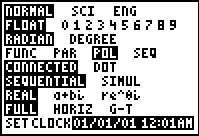
\includegraphics[width=1.8in]{./PolarGraphsGraphics/Polar01.jpg} &
\hspace{0.05in} 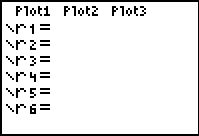
\includegraphics[width=1.8in]{./PolarGraphsGraphics/Polar02.jpg} & 
\hspace{0.05in} 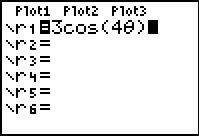
\includegraphics[width=1.8in]{./PolarGraphsGraphics/Polar03.jpg} \\

\end{tabular} 

\end{center}

This changes the ``Y='' menu as seen above in the middle.  Let's plot the polar rose given by $r = 3\cos(4\theta)$ from Exercise \ref{roseexercise8petal} above. We type the function into the ``r='' menu as seen above on the right.  We need to set the viewing window so that the curve displays properly, but when we look at the WINDOW menu, we find three extra lines.

\begin{center}

\begin{tabular}{cc}

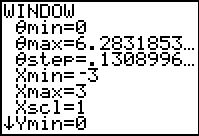
\includegraphics[width=1.8in]{./PolarGraphsGraphics/Polar04.jpg} &
\hspace{0.75in} 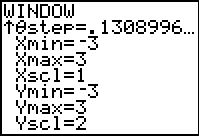
\includegraphics[width=1.8in]{./PolarGraphsGraphics/Polar05.jpg}\\

\end{tabular} 

\end{center}

In order for the calculator to be able to plot $r = 3\cos(4\theta)$ in the $xy$-plane, we need to tell it not only the dimensions which $x$ and $y$ will assume, but we also what values of $\theta$ to use.  From our previous work, we know that we need $0 \leq \theta \leq 2\pi$, so we enter the data you see above.  (I'll say more about the $\theta$-step in just a moment.)  Hitting GRAPH yields the curve below on the left which doesn't look quite right.  The issue here is that the calculator screen is 96 pixels wide but only 64 pixels tall.  To get a true geometric perspective, we need to hit ZOOM SQUARE (seen below in the middle) to produce a more accurate graph which we present below on the right.  

\begin{center}

\begin{tabular}{ccc}

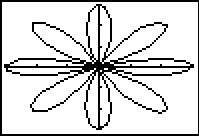
\includegraphics[width=1.8in]{./PolarGraphsGraphics/Polar06.jpg} &
\hspace{0.05in} 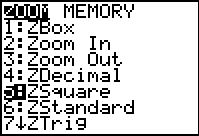
\includegraphics[width=1.8in]{./PolarGraphsGraphics/Polar07.jpg} & 
\hspace{0.05in} 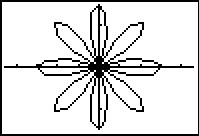
\includegraphics[width=1.8in]{./PolarGraphsGraphics/Polar08.jpg} \\

\end{tabular} 

\end{center}

In function mode, the calculator automatically divided the interval [Xmin, Xmax] into 96 equal subintervals.  In polar mode, however, we must specify how to split up the interval [$\theta$min, $\theta$max] using the $\theta$step.  For most graphs, a $\theta$step of 0.1 is fine.  If you make it too small then the calculator takes a long time to graph.  It you make it too big, you get chunky garbage like this.

\begin{center}

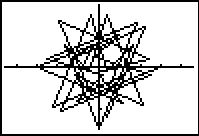
\includegraphics[width=1.8in]{./PolarGraphsGraphics/Polar09.jpg} 

\end{center}

You will need to experiment with the settings in order to get a nice graph.  Exercises \ref{polarcalcfirst} - \ref{polarcalclast} give you some curves to graph using your calculator.  Note some of them have explicit bounds on $\theta$ and others do not.

\begin{multicols}{2}

\begin{enumerate}

\setcounter{enumi}{\value{HW}}

\item $r = \theta, \, 0 \leq \theta \leq 12\pi$ \label{polarcalcfirst}
\item $r = \ln(\theta), \, 1 \leq \theta \leq 12\pi$

\setcounter{HW}{\value{enumi}}

\end{enumerate}

\end{multicols}

\begin{multicols}{2} 

\begin{enumerate}

\setcounter{enumi}{\value{HW}}

\item $r = e^{.1\theta}, \, 0 \leq \theta \leq 12\pi$
\item $r = \theta^{3} - \theta, \, -1.2 \leq \theta \leq 1.2$

\setcounter{HW}{\value{enumi}}

\end{enumerate}

\end{multicols}

\begin{multicols}{2} 

\begin{enumerate}

\setcounter{enumi}{\value{HW}}

\item $r = \sin(5\theta) - 3\cos(\theta)$
\item $r = \sin^{3}\left(\frac{\theta}{2}\right) + \cos^{2}\left(\frac{\theta}{3}\right)$

\setcounter{HW}{\value{enumi}}

\end{enumerate}

\end{multicols}

\begin{multicols}{2} 

\begin{enumerate}

\setcounter{enumi}{\value{HW}}

\item $r = \arctan(\theta), \, -\pi \leq \theta \leq \pi$ \vphantom{$\dfrac{1}{1 - \cos(\theta)}$} 
\item $r = \dfrac{1}{1 - \cos(\theta)}$

\setcounter{HW}{\value{enumi}}

\end{enumerate}

\end{multicols}

\begin{multicols}{2} 

\begin{enumerate}

\setcounter{enumi}{\value{HW}}

\item $r = \dfrac{1}{2 - \cos(\theta)}$
\item $r = \dfrac{1}{2 - 3\cos(\theta)}$ \label{polarcalclast}

\setcounter{HW}{\value{enumi}}

\end{enumerate}

\end{multicols}

\begin{enumerate}

\setcounter{enumi}{\value{HW}}

\item  Use a graphing utility to graph  $r = a - b \sin(\theta)$ for various (positive) values of $a$ and $b$.  Describe the shape of the curve when $a = b$, $a < b$, and when $a > b$.


\item How many petals does the polar rose $r = \sin(2\theta)$ have?  What about $r = \sin(3\theta)$, $r = \sin(4\theta)$ and $r = \sin(5\theta)$?  With the help of your classmates, make a conjecture as to how many petals the polar rose $r = \sin(n\theta)$ has for any natural number $n$.  Replace sine with cosine and repeat the investigation.  How many petals does $r = \cos(n\theta)$ have for each natural number $n$?  


\setcounter{HW}{\value{enumi}}

\end{enumerate}


Looking back through the graphs in the section, it's clear that many polar curves enjoy various forms of symmetry.  However, classifying symmetry for polar curves is not as straight-forward as it was for equations back in Section \ref{Relations}.  In Exercises \ref{sympolarfirst} - \ref{sympolarlast}, we have you and your classmates explore some of the more basic forms of symmetry seen in common polar curves.
\phantomsection
\label{polarsymmetry} 


\begin{enumerate}

\setcounter{enumi}{\value{HW}}

\item Show that if $f$ is even\footnote{Recall that this means $f(-\theta) = f(\theta)$ for $\theta$ in the domain of $f$.} then the graph of $r = f(\theta)$ is symmetric about the $x$-axis. \label{sympolarfirst}

\begin{enumerate}

\item Show that $f(\theta) = 2 + 4\cos(\theta)$ is even and verify that the graph of  $r = 2+4\cos(\theta)$ is indeed symmetric about the $x$-axis.  (See Example \ref{polargraphex} number \ref{limacon02}.)

\item Show that $f(\theta) = 3\sin\left(\frac{\theta}{2}\right)$ is \textbf{not} even, yet the graph of $r = 3\sin\left(\frac{\theta}{2}\right)$ \textbf{is} symmetric about the $x$-axis.  (See  Example \ref{polargraphintex} number \ref{samepolarcurveex}.) 

\end{enumerate}

\item  Show that if $f$ is odd\footnote{Recall that this means $f(-\theta) = -f(\theta)$ for $\theta$ in the domain of $f$.} then the graph of $r = f(\theta)$ is symmetric about the origin.

\begin{enumerate}

\item  Show that $f(\theta) = 5\sin(2\theta)$ is odd and verify that the graph of $r = 5\sin(2\theta)$ is indeed symmetric about the origin.  (See Example \ref{polargraphex} number \ref{rose}.)

\item  Show that $f(\theta) = 3\cos\left(\frac{\theta}{2}\right)$ is \textbf{not} odd, yet the graph of $r = 3\cos\left(\frac{\theta}{2}\right)$ \textbf{is} symmetric about the origin.  (See  Example \ref{polargraphintex} number \ref{samepolarcurveex}.)

\end{enumerate}

\newpage

\item  Show that if $ f(\pi-\theta)=f(\theta)$ for all $\theta$ in the domain of $f$ then the graph of $r = f(\theta)$ is symmetric about the $y$-axis. \label{sympolarlast}

\begin{enumerate}

\item  For $f(\theta) = 4-2\sin(\theta)$, show that $f(\pi - \theta) = f(\theta)$ and the graph of $r = 4-2\sin(\theta)$ is symmetric about the $y$-axis, as required.  (See Example \ref{polargraphex} number \ref{limacon01}.)

\item  For $f(\theta) = 5\sin(2\theta)$, show that $f\left(\pi - \frac{\pi}{4} \right) \neq  f\left(  \frac{\pi}{4} \right)$,  yet the graph of $r = 5\sin(2\theta)$ \textbf{is} symmetric about the $y$-axis.  (See  Example \ref{polargraphex} number  \ref{rose}.)

\end{enumerate}

\setcounter{HW}{\value{enumi}}

\end{enumerate}

In Section \ref{Transformations}, we discussed transformations of graphs.   In Exercise \ref{polargraphtransformations} we have you and your classmates explore transformations of polar graphs. 

\begin{enumerate}

\setcounter{enumi}{\value{HW}}

\item  For Exercises \ref{polargraphexercise1} and \ref{polargraphexercise2} below, let  $f(\theta) = \cos(\theta)$ and $g(\theta) = 2-\sin(\theta)$. \label{polargraphtransformations}

\begin{enumerate}

\item  Using a graphing utility, compare the graph of $r = f(\theta)$ to each of the graphs of $r = f\left(\theta  + \frac{\pi}{4}\right)$, $r = f\left(\theta  + \frac{3\pi}{4}\right)$, $r = f\left(\theta  - \frac{\pi}{4}\right)$ and $r = f\left(\theta  - \frac{3\pi}{4}\right)$.  Repeat this process for $g(\theta)$.  In general, how do you think the graph of $r = f(\theta + \alpha)$ compares with the graph of $r = f(\theta)$?
\label{polargraphexercise1}

\item  Using a graphing utility, compare the graph of $r = f(\theta)$ to each of the graphs of $r = 2f\left(\theta\right)$, $r = \frac{1}{2} f\left(\theta\right)$, $r = -f\left(\theta\right)$ and $r = -3 f(\theta)$.  Repeat this process for $g(\theta)$.  In general, how do you think the graph of $r = k \cdot f(\theta)$ compares with the graph of $r = f(\theta)$? 

Follow up question:  does it matter if $k>0$ or $k<0$?
\label{polargraphexercise2}

\end{enumerate}

\item In light of Exercises \ref{sympolarfirst} - \ref{sympolarlast}, how would the graph of $r = f(-\theta)$ compare with the graph of $r = f(\theta)$ for a generic function $f$?  What about the graphs of $r = -f(\theta)$ and $r = f(\theta)$?  What about $r = f(\theta)$ and $r = f(\pi - \theta)$?  Test out your conjectures using a variety of polar functions found in this section with the help of a graphing utility.

\setcounter{HW}{\value{enumi}}

\end{enumerate}


\begin{enumerate}

\setcounter{enumi}{\value{HW}}

\item With the help of your classmates, research cardioid microphones.

%\item Back in Section \ref{Relations}, in the paragraph before Exercise \ref{listofcurvesfirst}, we gave you this  \href{http://en.wikipedia.org/wiki/List_of_curves}{\underline{link}} to a fascinating list of curves.  Some of these curves have polar representations which we invite you and your classmates to research.

\setcounter{HW}{\value{enumi}}

\end{enumerate}

\newpage

\subsection{Answers}

\begin{multicols}{2} %\raggedcolumns

\begin{enumerate}

\item Circle: $r = 6\sin(\theta)$ 

\begin{mfpic}[15]{-5}{5}{-5}{5}
\axes
\tlabel[cc](5,-0.5){$x$}
\tlabel[cc](0.5,5){$y$}
\xmarks{-4,4}
\ymarks{-4,4}
\tlpointsep{4pt}
\scriptsize
\axislabels {x}{{$-6 \hspace{6pt}$} -4, {$6$} 4}
\axislabels {y}{{$-6$} -4, {$6$} 4}
\normalsize
\penwd{1.25pt}
\plrfcn{0,180,5}{4*sind t}
\end{mfpic} 

\item Circle: $r = 2\cos(\theta)$ 

\begin{mfpic}[15]{-5}{5}{-5}{5}
\axes
\tlabel[cc](5,-0.5){$x$}
\tlabel[cc](0.5,5){$y$}
\xmarks{-4,4}
\ymarks{-4,4}
\tlpointsep{4pt}
\scriptsize
\axislabels {x}{{$-2 \hspace{6pt}$} -4, {$2$} 4}
\axislabels {y}{{$-2$} -4, {$2$} 4}
\normalsize
\penwd{1.25pt}
\plrfcn{0,180,5}{4*cosd t}
\end{mfpic} 

\setcounter{HW}{\value{enumi}}

\end{enumerate}

\end{multicols}

\begin{multicols}{2} 

\begin{enumerate}

\setcounter{enumi}{\value{HW}}

\item Rose: $r = 2\sin(2\theta)$ 

\begin{mfpic}[15]{-5}{5}{-5}{5}
\axes
\tlabel[cc](5,-0.5){$x$}
\tlabel[cc](0.5,5){$y$}
\xmarks{-4,4}
\ymarks{-4,4}
\tlpointsep{4pt}
\scriptsize
\axislabels {x}{{$-2 \hspace{6pt}$} -4, {$2$} 4}
\axislabels {y}{{$-2$} -4, {$2$} 4}
\normalsize
\penwd{1.25pt}
\plrfcn{0,360,5}{4*sind(2*t)}
\end{mfpic} 

\item Rose: $r = 4\cos(2\theta)$ 

\begin{mfpic}[15]{-5}{5}{-5}{5}
\axes
\tlabel[cc](5,-0.5){$x$}
\tlabel[cc](0.5,5){$y$}
\xmarks{-4,4}
\ymarks{-4,4}
\tlpointsep{4pt}
\scriptsize
\axislabels {x}{{$-4 \hspace{6pt}$} -4, {$4$} 4}
\axislabels {y}{{$-4$} -4, {$4$} 4}
\normalsize
\dashed \polyline{(3,3), (-3,-3)}
\gclear \tlabelrect(3,3){\scriptsize $\theta = \frac{\pi}{4}$}
\dashed \polyline{(3,-3), (-3,3)}
\gclear \tlabelrect(-3,3){\scriptsize $\theta = \frac{3\pi}{4}$}
\penwd{1.25pt}
\plrfcn{0,360,5}{4*cosd(2*t)}
\end{mfpic} 

\setcounter{HW}{\value{enumi}}

\end{enumerate}

\end{multicols}

\begin{multicols}{2} 

\begin{enumerate}

\setcounter{enumi}{\value{HW}}

\item Rose: $r = 5\sin(3\theta)$ 

\begin{mfpic}[15]{-5}{5}{-5}{5}
\axes
\tlabel[cc](5,-0.5){$x$}
\tlabel[cc](0.5,5){$y$}
\xmarks{-4,4}
\ymarks{-4,4}
\tlpointsep{4pt}
\scriptsize
\axislabels {x}{{$-5 \hspace{6pt}$} -4, {$5$} 4}
\axislabels {y}{{$-5$} -4, {$5$} 4}
\normalsize
\dashed \polyline{(2,3.464), (-2,-3.464)}
\gclear \tlabelrect(2,3.464){\scriptsize $\theta = \frac{\pi}{3}$}
\dashed \polyline{(-2,3.464), (2,-3.464)}
\gclear \tlabelrect(-2,3.464){\scriptsize $\theta = \frac{2\pi}{3}$}
\penwd{1.25pt}
\plrfcn{0,180,5}{4*sind(3*t)}
\end{mfpic} 

\item Rose: $r = \cos(5\theta)$ 

\begin{mfpic}[15]{-5}{5}{-5}{5}
\axes
\tlabel[cc](5,-0.5){$x$}
\tlabel[cc](0.5,5){$y$}
\xmarks{-4,4}
\ymarks{-4,4}
\tlpointsep{4pt}
\scriptsize
\axislabels {x}{{$-1 \hspace{6pt}$} -4, {$1$} 4}
\axislabels {y}{{$-1$} -4, {$1$} 4}
\normalsize
\dashed \polyline{(3.804,1.236), (-3.804,-1.236)}
\gclear \tlabelrect(3.804,1.236){\scriptsize $\theta = \frac{\pi}{10}$}
\dashed \polyline{(2.351,3.236), (-2.351,-3.236)}
\gclear \tlabelrect(2.351,3.236){\scriptsize $\theta = \frac{3\pi}{10}$}
\dashed \polyline{(-2.351,3.236), (2.351,-3.236)}
\gclear \tlabelrect(-2.351,3.236){\scriptsize $\theta = \frac{7\pi}{10}$}
\dashed \polyline{(-3.804,1.236), (3.804,-1.236)}
\gclear \tlabelrect(-3.804,1.236){\scriptsize $\theta = \frac{9\pi}{10}$}
\penwd{1.25pt}
\plrfcn{0,180,5}{4*cosd(5*t)}
\end{mfpic} 

\setcounter{HW}{\value{enumi}}

\end{enumerate}

\end{multicols}

\begin{multicols}{2} 

\begin{enumerate}

\setcounter{enumi}{\value{HW}}

\item Rose: $r = \sin(4\theta)$ 

\begin{mfpic}[15]{-5}{5}{-5}{5}
\axes
\tlabel[cc](5,-0.5){$x$}
\tlabel[cc](0.5,5){$y$}
\xmarks{-4,4}
\ymarks{-4,4}
\tlpointsep{4pt}
\scriptsize
\axislabels {x}{{$-1 \hspace{6pt}$} -4, {$1$} 4}
\axislabels {y}{{$-1$} -4, {$1$} 4}
\normalsize
\dashed \polyline{(3,3), (-3,-3)}
\gclear \tlabelrect(3,3){\scriptsize $\theta = \frac{\pi}{4}$}
\dashed \polyline{(3,-3), (-3,3)}
\gclear \tlabelrect(-3,3){\scriptsize $\theta = \frac{3\pi}{4}$}
\penwd{1.25pt}
\plrfcn{0,360,5}{4*sind(4*t)}
\end{mfpic} 

\item Rose: $r = 3\cos(4\theta)$ 

\begin{mfpic}[15]{-5}{5}{-5}{5}
\axes
\tlabel[cc](5,-0.5){$x$}
\tlabel[cc](0.5,5){$y$}
\xmarks{-4,4}
\ymarks{-4,4}
\tlpointsep{4pt}
\scriptsize
\axislabels {x}{{$-3 \hspace{6pt}$} -4, {$3$} 4}
\axislabels {y}{{$-3$} -4, {$3$} 4}
\normalsize
\dashed \polyline{(3.696,1.531), (-3.696,-1.531)}
\gclear \tlabelrect(3.696,1.531){\scriptsize $\theta = \frac{\pi}{8}$}
\dashed \polyline{(1.531,3.696), (-1.531,-3.696)}
\gclear \tlabelrect(1.531,3.696){\scriptsize $\theta = \frac{3\pi}{8}$}
\dashed \polyline{(-1.531,3.696), (1.531,-3.696)}
\gclear \tlabelrect(-1.531,3.696){\scriptsize $\theta = \frac{5\pi}{8}$}
\dashed \polyline{(-3.696,1.531), (3.696,-1.531)}
\gclear \tlabelrect(-3.696,1.531){\scriptsize $\theta = \frac{7\pi}{8}$}
\penwd{1.25pt}
\plrfcn{0,360,5}{4*cosd(4*t)}
\end{mfpic} 

\setcounter{HW}{\value{enumi}}

\end{enumerate}

\end{multicols}

\begin{multicols}{2} 

\begin{enumerate}

\setcounter{enumi}{\value{HW}}

\item Cardioid: $r = 3 - 3\cos(\theta)$ 

\begin{mfpic}[15]{-5}{5}{-5}{5}
\axes
\tlabel[cc](5,-0.5){$x$}
\tlabel[cc](0.5,5){$y$}
\xmarks{-4,-2,2,4}
\ymarks{-4,-2,2,4}
\tlpointsep{4pt}
\scriptsize
\axislabels {x}{{$-6 \hspace{6pt}$} -4, {$-3 \hspace{6pt}$} -2, {$3$} 2, {$6$} 4}
\axislabels {y}{{$-6$} -4, {$-3$} -2, {$3$} 2, {$6$} 4}
\normalsize
\penwd{1.25pt}
\plrfcn{0,360,5}{2 - 2*cosd(t)}
\end{mfpic} 

\item Cardioid: $r = 5 + 5\sin(\theta)$ 

\begin{mfpic}[15]{-5}{5}{-5}{5}
\axes
\tlabel[cc](5,-0.5){$x$}
\tlabel[cc](0.5,5){$y$}
\xmarks{-4,-2,2,4}
\ymarks{-4,-2,2,4}
\tlpointsep{4pt}
\scriptsize
\axislabels {x}{{$-10 \hspace{6pt}$} -4, {$-5 \hspace{6pt}$} -2, {$5$} 2, {$10$} 4}
\axislabels {y}{{$-10$} -4, {$-5$} -2, {$5$} 2, {$10$} 4}
\normalsize
\penwd{1.25pt}
\plrfcn{0,360,5}{2 + 2*sind(t)}
\end{mfpic} 

\setcounter{HW}{\value{enumi}}

\end{enumerate}

\end{multicols}

\begin{multicols}{2} 

\begin{enumerate}

\setcounter{enumi}{\value{HW}}

\item Cardioid: $r = 2 + 2\cos(\theta)$ 

\begin{mfpic}[15]{-5}{5}{-5}{5}
\axes
\tlabel[cc](5,-0.5){$x$}
\tlabel[cc](0.5,5){$y$}
\xmarks{-4,-2,2,4}
\ymarks{-4,-2,2,4}
\tlpointsep{4pt}
\scriptsize
\axislabels {x}{{$-4 \hspace{6pt}$} -4, {$-2 \hspace{6pt}$} -2, {$2$} 2, {$4$} 4}
\axislabels {y}{{$-4$} -4, {$-2$} -2, {$2$} 2, {$4$} 4}
\normalsize
\penwd{1.25pt}
\plrfcn{0,360,5}{2 + 2*cosd(t)}
\end{mfpic} 

\item Cardioid: $r = 1 - \sin(\theta)$ 

\begin{mfpic}[15]{-5}{5}{-5}{5}
\axes
\tlabel[cc](5,-0.5){$x$}
\tlabel[cc](0.5,5){$y$}
\xmarks{-4,-2,2,4}
\ymarks{-4,-2,2,4}
\tlpointsep{4pt}
\scriptsize
\axislabels {x}{{$-2 \hspace{6pt}$} -4, {$-1 \hspace{6pt}$} -2, {$1$} 2, {$2$} 4}
\axislabels {y}{{$-2$} -4, {$-1$} -2, {$1$} 2, {$2$} 4}
\normalsize
\penwd{1.25pt}
\plrfcn{0,360,5}{2 - 2*sind(t)}
\end{mfpic} 

\setcounter{HW}{\value{enumi}}

\end{enumerate}

\end{multicols}

\begin{multicols}{2} 

\begin{enumerate}

\setcounter{enumi}{\value{HW}}

\item Lima\c{c}on: $r = 1 - 2\cos(\theta)$ 

\begin{mfpic}[15]{-5}{5}{-5}{5}
\axes
\tlabel[cc](5,-0.5){$x$}
\tlabel[cc](0.5,5){$y$}
\xmarks{-4,-1.3333,1.3333,4}
\ymarks{-4,-1.3333,1.3333,4}
\tlpointsep{4pt}
\scriptsize
\axislabels {x}{{$-3 \hspace{6pt}$} -4, {$-1 \hspace{6pt}$} -1.3333, {$1$} 1.3333, {$3$} 4}
\axislabels {y}{{$-3$} -4, {$-1$} -1.3333, {$1$} 1.3333, {$3$} 4}
\normalsize
\dashed \polyline{(0,0), (2,3.464)}
\gclear \tlabelrect(2,3.464){\scriptsize $\theta = \frac{\pi}{3}$}
\dashed \polyline{(0,0), (2,-3.464)}
\gclear \tlabelrect(2,-3.464){\scriptsize $\theta = \frac{5\pi}{3}$}
\penwd{1.25pt}
\plrfcn{0,360,5}{1.3333*(1 - 2*cosd(t))}
\end{mfpic} 

\item Lima\c{c}on: $r = 1 - 2\sin(\theta)$ 

\begin{mfpic}[15]{-5}{5}{-5}{5}
\axes
\tlabel[cc](5,-0.5){$x$}
\tlabel[cc](0.5,5){$y$}
\xmarks{-4,-1.3333,1.3333,4}
\ymarks{-4,-1.3333,1.3333,4}
\tlpointsep{4pt}
\scriptsize
\axislabels {x}{{$-3 \hspace{6pt}$} -4, {$-1 \hspace{6pt}$} -1.3333, {$1$} 1.3333, {$3$} 4}
\axislabels {y}{{$-3$} -4, {$-1$} -1.3333, {$1$} 1.3333, {$3$} 4}
\normalsize
\dashed \polyline{(0,0), (3.464,2)}
\gclear \tlabelrect(3.464,2){\scriptsize $\theta = \frac{\pi}{6}$}
\dashed \polyline{(0,0), (-3.464,2)}
\gclear \tlabelrect(-3.464,2){\scriptsize $\theta = \frac{5\pi}{6}$}
\penwd{1.25pt}
\plrfcn{0,360,5}{1.3333*(1 - 2*sind(t))}
\end{mfpic} 

\setcounter{HW}{\value{enumi}}

\end{enumerate}

\end{multicols}

\begin{multicols}{2} 

\begin{enumerate}

\setcounter{enumi}{\value{HW}}

\item Lima\c{c}on: $r = 2\sqrt{3} + 4\cos(\theta)$ 

\begin{mfpic}[15]{-5}{5}{-5}{5}
\axes
\tlabel[cc](5,0.5){$x$}
\tlabel[cc](0.5,5){$y$}
\xmarks{-4,-1.856,1.856,4}
\ymarks{-4,4}
\tlpointsep{4pt}
\scriptsize
\axislabels {x}{{$-2\sqrt{3} - 4 \hspace{6pt}$} -4, {$2\sqrt{3} + 4$} 4}
\axislabels {y}{{$-2\sqrt{3} - 4$} -4, {$-2\sqrt{3}$} -1.856, {$2\sqrt{3}$} 1.856, {$2\sqrt{3} + 4$} 4}
\normalsize
\dashed \polyline{(0,0), (-3.464,-2)}
\gclear \tlabelrect(-3.464,-2){\scriptsize $\theta = \frac{7\pi}{6}$}
\dashed \polyline{(0,0), (-3.464,2)}
\gclear \tlabelrect(-3.464,2){\scriptsize $\theta = \frac{5\pi}{6}$}
\penwd{1.25pt}
\plrfcn{0,360,5}{1.0718*(1.73205 + 2*cosd(t))}
\end{mfpic} 

\item Lima\c{c}on: $r = 3-5\cos(\theta)$ 

\begin{mfpic}[15]{-5}{5}{-5}{5}
\axes
\tlabel[cc](5,-0.5){$x$}
\tlabel[cc](0.5,5){$y$}
\xmarks{-4,-1,4}
\ymarks{-4,-1.5,1.5,4}
\tlpointsep{4pt}
\scriptsize
\axislabels {y}{{$-8$} -4, {$-3$} -1.5, {$3$} 1.5, {$8$} 4}
\axislabels {x}{{$-8 \hspace{6pt}$} -4, {$-2 \hspace{6pt}$} -1, {$8$} 4}
\normalsize
\dashed \polyline{(0,0), (2.41,3.19)}
\gclear \tlabelrect(2.9,3.3){\tiny $\theta = \arccos\left(\frac{3}{5}\right)$}
\dashed \polyline{(0,0), (2.41,-3.19)}
\gclear \tlabelrect(2.9,-3.3){\tiny $\theta = 2\pi - \arccos\left(\frac{3}{5}\right)$}
\penwd{1.25pt}
\plrfcn{0,360,5}{0.5*(3 - 5*cosd(t))}
\end{mfpic} 

\setcounter{HW}{\value{enumi}}

\end{enumerate}

\end{multicols}

\begin{multicols}{2} 

\begin{enumerate}

\setcounter{enumi}{\value{HW}}

\item Lima\c{c}on: $r = 3-5\sin(\theta)$ 

\begin{mfpic}[15]{-5}{5}{-5}{5}
\axes
\tlabel[cc](5,-0.5){$x$}
\tlabel[cc](0.5,5){$y$}
\xmarks{-4,-1.5,1.5,4}
\ymarks{-4,-1,4}
\tlpointsep{4pt}
\scriptsize
\axislabels {x}{{$-8 \hspace{6pt}$} -4, {$-3 \hspace{6pt}$} -1.5, {$3$} 1.5, {$8$} 4}
\axislabels {y}{{$-8$} -4, {$-2$} -1, {$8$} 4}
\normalsize
\dashed \polyline{(0,0), (3.2,2.4)}
\gclear \tlabelrect(2.9,3){\tiny $\theta = \arcsin\left(\frac{3}{5}\right)$}
\dashed \polyline{(0,0), (-3.2,2.4)}
\gclear \tlabelrect(-2.9,3){\tiny $\theta = \pi - \arcsin\left(\frac{3}{5}\right)$}
\penwd{1.25pt}
\plrfcn{0,360,5}{0.5*(3 - 5*sind(t))}
\end{mfpic} 

\item Lima\c{c}on: $r = 2 + 7\sin(\theta)$ 

\begin{mfpic}[15]{-5}{5}{-5}{5}
\axes
\tlabel[cc](5,-0.5){$x$}
\tlabel[cc](0.5,5){$y$}
\xmarks{-4,-0.8888,0.8888,4}
\ymarks{-4,2.2222,4}
\tlpointsep{4pt}
\scriptsize
\axislabels {x}{{$-9 \hspace{6pt}$} -4, {$-2 \hspace{6pt}$} -0.8888, {$2$} 0.8888, {$9$} 4}
\axislabels {y}{{$-9$} -4, {$5$} 2.2222, {$9$} 4}
\normalsize
\dashed \polyline{(0,0), (-3.842,-1.113)}
\gclear \tlabelrect(-2.9,-1.3){\tiny $\theta = \pi + \arcsin\left(\frac{2}{7}\right)$}
\dashed \polyline{(0,0), (3.842,-1.113)}
\gclear \tlabelrect(2.9,-1.3){\tiny $\theta = 2\pi - \arcsin\left(\frac{2}{7}\right)$}
\penwd{1.25pt}
\plrfcn{0,360,5}{0.4444*(2 + 7*sind(t))}
\end{mfpic} 

\setcounter{HW}{\value{enumi}}

\end{enumerate}

\end{multicols}

\begin{multicols}{2} 

\begin{enumerate}

\setcounter{enumi}{\value{HW}}

\item Lemniscate: $r^{2} = \sin(2\theta)$ 

\begin{mfpic}[15]{-5}{5}{-5}{5}
\axes
\tlabel[cc](5,-0.5){$x$}
\tlabel[cc](0.5,5){$y$}
\xmarks{-4,4}
\ymarks{-4,4}
\tlpointsep{4pt}
\scriptsize
\axislabels {x}{{$-1 \hspace{6pt}$} -4, {$1$} 4}
\axislabels {y}{{$-1$} -4, {$1$} 4}
\normalsize
\penwd{1.25pt}
\plrfcn{0,90,5}{4*sqrt(sind(2*t))}
\plrfcn{180,270,5}{4*sqrt(sind(2*t))}
\end{mfpic} 

\item Lemniscate: $r^{2} = 4\cos(2\theta)$ 

\begin{mfpic}[15]{-5}{5}{-5}{5}
\axes
\tlabel[cc](5,-0.5){$x$}
\tlabel[cc](0.5,5){$y$}
\xmarks{-4,4}
\ymarks{-4,4}
\tlpointsep{4pt}
\scriptsize
\axislabels {x}{{$-2 \hspace{6pt}$} -4, {$2$} 4}
\axislabels {y}{{$-2$} -4, {$2$} 4}
\normalsize
\dashed \polyline{(3,3), (-3,-3)}
\gclear \tlabelrect(3,3){\scriptsize $\theta = \frac{\pi}{4}$}
\dashed \polyline{(3,-3), (-3,3)}
\gclear \tlabelrect(-3,3){\scriptsize $\theta = \frac{3\pi}{4}$}
\penwd{1.25pt}
\plrfcn{-45,45,5}{4*sqrt(cosd(2*t))}
\plrfcn{135,225,5}{4*sqrt(cosd(2*t))}
\end{mfpic} 

\setcounter{HW}{\value{enumi}}

\end{enumerate}

\end{multicols}

\begin{enumerate}

\setcounter{enumi}{\value{HW}}

\item \begin{multicols}{2} \raggedcolumns

$r = 3\cos(\theta)$ and $r = 1 + \cos(\theta)$

\begin{mfpic}[17]{-4}{4}{-4}{4}
\axes
\tlabel[cc](4,-0.5){$x$}
\tlabel[cc](0.5,4){$y$}
\xmarks{-3,-2,-1,1,2,3}
\ymarks{-3,-2,-1,1,2,3}
\tlpointsep{4pt}
\scriptsize
\axislabels {x}{{$-3 \hspace{6pt}$} -3, {$-2 \hspace{6pt}$} -2, {$-1 \hspace{6pt}$} -1, {$1$} 1, {$2$} 2, {$3$} 3}
\axislabels {y}{{$-3$} -3, {$-2$} -2, {$-1$} -1, {$1$} 1, {$2$} 2, {$3$} 3}
\normalsize
\penwd{1.25pt}
\plrfcn{0,360,5}{1 + cosd(t)}
\plrfcn{0,360,5}{3*cosd(t)}
\end{mfpic} 

$\left( \dfrac{3}{2}, \dfrac{\pi}{3} \right)$, $\left( \dfrac{3}{2}, \dfrac{5\pi}{3} \right)$, pole

\end{multicols}

\item \begin{multicols}{2} \raggedcolumns 

$r = 1 + \sin(\theta)$ and $r = 1 - \cos(\theta)$

\begin{mfpic}[23]{-2.9}{3}{-3}{3}
\axes
\tlabel[cc](3,-0.5){$x$}
\tlabel[cc](0.5,3){$y$}
\xmarks{-2,-1,1,2}
\ymarks{-2,-1,1,2}
\tlpointsep{4pt}
\scriptsize
\axislabels {x}{{$-2 \hspace{6pt}$} -2, {$-1 \hspace{6pt}$} -1, {$1$} 1, {$2$} 2}
\axislabels {y}{{$-2$} -2, {$-1$} -1, {$1$} 1, {$2$} 2}
\normalsize
\penwd{1.25pt}
\plrfcn{0,360,5}{1 - cosd(t)}
\plrfcn{0,360,5}{1 + sind(t)}
\end{mfpic} 

$\left( \dfrac{2 + \sqrt{2}}{2}, \dfrac{3\pi}{4} \right)$, $\left( \dfrac{2 - \sqrt{2}}{2}, \dfrac{7\pi}{4} \right)$, pole

\end{multicols}

\pagebreak

\item \begin{multicols}{2} \raggedcolumns 

$r = 1 - 2\sin(\theta)$ and $r = 2$

\begin{mfpic}[15]{-5}{5}{-5}{5}
\axes
\tlabel[cc](5,-0.5){$x$}
\tlabel[cc](0.5,5){$y$}
\xmarks{-4,-1.3333,1.3333,4}
\ymarks{-4,-1.3333,1.3333,4}
\tlpointsep{4pt}
\scriptsize
\axislabels {x}{{$-3 \hspace{6pt}$} -4, {$-1 \hspace{6pt}$} -1.3333, {$1$} 1.3333, {$3$} 4}
\axislabels {y}{{$-3$} -4, {$-1$} -1.3333, {$1$} 1.3333, {$3$} 4}
\normalsize
\penwd{1.25pt}
\plrfcn{0,360,5}{1.3333*(1 - 2*sind(t))}
\circle{(0,0),2}
\end{mfpic} 

$\left( 2, \dfrac{7\pi}{6} \right)$, $\left( 2, \dfrac{11\pi}{6} \right)$

\end{multicols}

\item \begin{multicols}{2} \raggedcolumns 

$r = 1 - 2\cos(\theta)$ and $r = 1$

\begin{mfpic}[15]{-5}{5}{-5}{5}
\axes
\tlabel[cc](5,-0.5){$x$}
\tlabel[cc](0.5,5){$y$}
\xmarks{-4,-1.3333,1.3333,4}
\ymarks{-4,-1.3333,1.3333,4}
\tlpointsep{4pt}
\scriptsize
\axislabels {x}{{$-3 \hspace{6pt}$} -4, {$-1 \hspace{6pt}$} -1.3333, {$1$} 1.3333, {$3$} 4}
\axislabels {y}{{$-3$} -4, {$-1$} -1.3333, {$1$} 1.3333, {$3$} 4}
\normalsize
\penwd{1.25pt}
\plrfcn{0,360,5}{1.3333*(1 - 2*cosd(t))}
\plrfcn{0,360,5}{1.3333}
\end{mfpic} 

$\left( 1, \dfrac{\pi}{2} \right)$, $\left( 1, \dfrac{3\pi}{2} \right)$, $(-1, 0)$

\end{multicols}

\item \begin{multicols}{2} \raggedcolumns  

$r = 2\cos(\theta)$ and $r = 2\sqrt{3} \sin(\theta)$

\begin{mfpic}[19]{-4}{4}{-5}{5}
\axes
\tlabel[cc](4,-0.5){$x$}
\tlabel[cc](0.5,5){$y$}
\xmarks{-3,-2,-1,1,2,3}
\ymarks{-4,-3,-2,-1,1,2,3,4}
\tlpointsep{4pt}
\scriptsize
\axislabels {x}{{$-3 \hspace{6pt}$} -3, {$-2 \hspace{6pt}$} -2, {$-1 \hspace{6pt}$} -1, {$1$} 1, {$2$} 2, {$3$} 3}
\axislabels {y}{{$-4$} -4,{$-3$} -3, {$-2$} -2, {$-1$} -1, {$1$} 1, {$2$} 2, {$3$} 3, {$4$} 4}
\normalsize
\penwd{1.25pt}
\plrfcn{0,360,5}{3.46*sind(t)}
\plrfcn{0,360,5}{2*cosd(t)}
\end{mfpic} 

$\left(\sqrt{3}, \dfrac{\pi}{6} \right)$, pole

\end{multicols}


\item \begin{multicols}{2} \raggedcolumns  

$r = 3\cos(\theta)$ and $r = \sin(\theta)$

\begin{mfpic}[19]{-4}{4}{-4}{4}
\axes
\tlabel[cc](4,-0.5){$x$}
\tlabel[cc](0.5,4){$y$}
\xmarks{-3,-2,-1,1,2,3}
\ymarks{-3,-2,-1,1,2,3}
\tlpointsep{4pt}
\scriptsize
\axislabels {x}{{$-3 \hspace{6pt}$} -3, {$-2 \hspace{6pt}$} -2, {$-1 \hspace{6pt}$} -1, {$1$} 1, {$2$} 2, {$3$} 3}
\axislabels {y}{{$-3$} -3, {$-2$} -2, {$-1$} -1, {$1$} 1, {$2$} 2, {$3$} 3}
\normalsize
\penwd{1.25pt}
\plrfcn{0,360,5}{sind(t)}
\plrfcn{0,360,5}{3*cosd(t)}
\end{mfpic} 

$\left(\dfrac{3\sqrt{10}}{10}, \arctan(3)\right)$, pole

\end{multicols}

\item \begin{multicols}{2} \raggedcolumns 

$r^2 = 4\cos(2\theta)$ and $r = \sqrt{2}$

\begin{mfpic}[15]{-5}{5}{-5}{5}
\axes
\tlabel[cc](5,-0.5){$x$}
\tlabel[cc](0.5,5){$y$}
\xmarks{-4,4}
\ymarks{-4,4}
\tlpointsep{4pt}
\scriptsize
\axislabels {x}{{$-2 \hspace{6pt}$} -4, {$2$} 4}
\axislabels {y}{{$-2$} -4, {$2$} 4}
\normalsize
\penwd{1.25pt}
\plrfcn{-45,45,5}{4*sqrt(cosd(2*t))}
\plrfcn{135,225,5}{4*sqrt(cosd(2*t))}
\circle{(0,0), 1.414}

\end{mfpic} 

$\left(\sqrt{2}, \dfrac{\pi}{6}\right)$, $\left(\sqrt{2}, \dfrac{5\pi}{6}\right)$, $\left(\sqrt{2}, \dfrac{7\pi}{6}\right)$, $\left(\sqrt{2}, \dfrac{11\pi}{6}\right)$

\end{multicols}

\item \begin{multicols}{2} \raggedcolumns 

$r^{2} = 2\sin(2\theta)$ and $r = 1$

\begin{mfpic}[15]{-5}{5}{-5}{5}
\axes
\tlabel[cc](5,-0.5){$x$}
\tlabel[cc](0.5,5){$y$}
\xmarks{-4,4}
\ymarks{-4,4}
\tlpointsep{4pt}
\scriptsize
\axislabels {x}{{\tiny $-\sqrt{2} \hspace{6pt}$} -4, {$-1 \hspace{6pt}$} -2.828, {$1$} 2.828, {\tiny $\sqrt{2}$} 4}
\axislabels {y}{{\tiny $-\sqrt{2}$} -4, {$-1$} -2.828, {$1$} 2.828, {\tiny $\sqrt{2}$} 4}
\normalsize
\penwd{1.25pt}
\plrfcn{0,90,5}{4*sqrt(sind(2*t))}
\plrfcn{180,270,5}{4*sqrt(sind(2*t))}
\plrfcn{0,360,5}{2.828}
\end{mfpic} 

$\left(1, \dfrac{\pi}{12}\right)$, $\left(1, \dfrac{5\pi}{12}\right)$, $\left(1, \dfrac{13\pi}{12}\right)$, $\left(1, \dfrac{17\pi}{12}\right)$

\end{multicols}

\pagebreak

\item \begin{multicols}{2} \raggedcolumns

 $r = 4\cos(2\theta)$  and $r = 2$

\begin{mfpic}[15]{-5}{5}{-5}{5}
\axes
\tlabel[cc](5,-0.5){$x$}
\tlabel[cc](0.5,5){$y$}
\xmarks{-4,4}
\ymarks{-4,4}
\tlpointsep{4pt}
\scriptsize
\axislabels {x}{{$-4 \hspace{6pt}$} -4, {$4$} 4}
\axislabels {y}{{$-4$} -4, {$4$} 4}
\normalsize
\penwd{1.25pt}
\plrfcn{0,360,5}{4*cosd(2*t)}
\circle{(0,0),2}

\end{mfpic} 

$\left( 2, \dfrac{\pi}{6} \right)$, $\left( 2, \dfrac{5\pi}{6} \right)$, $\left( 2, \dfrac{7\pi}{6} \right)$, 

$\left( 2, \dfrac{11\pi}{6} \right)$, $\left( -2, \dfrac{\pi}{3} \right)$, $\left( -2, \dfrac{2\pi}{3} \right)$, 

$\left( -2, \dfrac{4\pi}{3} \right)$, $\left( -2, \dfrac{5\pi}{3} \right)$

\end{multicols}

\item \begin{multicols}{2} \raggedcolumns

$r = 2\sin(2\theta)$ and $r = 1$

\begin{mfpic}[15]{-4.5}{5}{-5}{5}
\axes
\tlabel[cc](5,-0.5){$x$}
\tlabel[cc](0.5,5){$y$}
\xmarks{-4,4}
\ymarks{-4,4}
\tlpointsep{4pt}
\scriptsize
\axislabels {x}{{$-2 \hspace{6pt}$} -4, {$2$} 4}
\axislabels {y}{{$-2$} -4, {$2$} 4}
\normalsize
\penwd{1.25pt}
\plrfcn{0,360,5}{4*sind(2*t)}
\plrfcn{0,360,5}{2}
\end{mfpic} 

$\left( 1, \dfrac{\pi}{12} \right)$, $\left( 1, \dfrac{5\pi}{12} \right)$, $\left( 1, \dfrac{13\pi}{12} \right)$, 

$\left( 1, \dfrac{17\pi}{12} \right)$, $\left( -1, \dfrac{7\pi}{12} \right)$, $\left( -1, \dfrac{11\pi}{12} \right)$, 

$\left( -1, \dfrac{19\pi}{12} \right)$, $\left( -1, \dfrac{23\pi}{12} \right)$

\end{multicols}

\setcounter{HW}{\value{enumi}}

\end{enumerate}

\pagebreak

\begin{multicols}{2}

\begin{enumerate}

\setcounter{enumi}{\value{HW}}

\item $\left\{ (r,\theta) \, | \, 0 \leq r \leq 3, \,0 \leq \theta \leq 2\pi \right\}$

\begin{mfpic}[15]{-5}{5}{-5}{5}
\fillcolor[gray]{0.7}
\gfill \circle{(0,0),3}
\axes
\tlabel[cc](5,-0.5){$x$}
\tlabel[cc](0.5,5){$y$}
\xmarks{-3,-2,-1,1,2,3}
\ymarks{-3,-2,-1,1,2,3}
\tlpointsep{4pt}
\scriptsize
\axislabels {x}{{$-3 \hspace{6pt}$} -3, {$-2 \hspace{6pt}$} -2, {$-1 \hspace{6pt}$} -1, {$1$} 1, {$2$} 2, {$3$} 3}
\axislabels {y}{{$-3$} -3, {$-2$} -2, {$-1$} -1, {$1$} 1, {$2$} 2, {$3$} 3}
\normalsize
\penwd{1.25pt}
\circle{(0,0),3}
\end{mfpic} 

\item $\left\{ (r,\theta) \, | \, 0 \leq r \leq 4\sin(\theta), \,0 \leq \theta \leq \pi \right\}$

\begin{mfpic}[15]{-5}{5}{-5}{5}
\fillcolor[gray]{0.7}
\gfill \plrregion{0,180,1}{4*sind(t)}
\axes
\tlabel[cc](5,-0.5){$x$}
\tlabel[cc](0.5,5){$y$}
\xmarks{-4,-3,-2,-1,1,2,3,4}
\ymarks{-4,-3,-2,-1,1,2,3,4}
\tlpointsep{4pt}
\scriptsize
\axislabels {x}{{$-4 \hspace{6pt}$} -4,{$-3 \hspace{6pt}$} -3, {$-2 \hspace{6pt}$} -2, {$-1 \hspace{6pt}$} -1, {$1$} 1, {$2$} 2, {$3$} 3, {$4$} 4}
\axislabels {y}{{$-4$} -4,{$-3$} -3, {$-2$} -2, {$-1$} -1, {$1$} 1, {$2$} 2, {$3$} 3, {$4$} 4}
\normalsize
\penwd{1.25pt}
\plrfcn{0,180,5}{4*sind(t)}
\end{mfpic} 

\setcounter{HW}{\value{enumi}}

\end{enumerate}

\end{multicols}

\begin{multicols}{2} 

\begin{enumerate}

\setcounter{enumi}{\value{HW}}

\item $\left\{ (r,\theta) \, | \, 0 \leq r \leq 3\cos(\theta), \, -\frac{\pi}{2} \leq \theta \leq \frac{\pi}{2} \right\}$

\begin{mfpic}[15]{-5}{5}{-5}{5}
\fillcolor[gray]{0.7}
\gfill \plrregion{-90,90,1}{3*cosd(t)}
\axes
\tlabel[cc](5,-0.5){$x$}
\tlabel[cc](0.5,5){$y$}
\xmarks{-3,-2,-1,1,2,3}
\ymarks{-3,-2,-1,1,2,3}
\tlpointsep{4pt}
\scriptsize
\axislabels {x}{{$-3 \hspace{6pt}$} -3, {$-2 \hspace{6pt}$} -2, {$-1 \hspace{6pt}$} -1, {$1$} 1, {$2$} 2, {$3$} 3}
\axislabels {y}{{$-3$} -3, {$-2$} -2, {$-1$} -1, {$1$} 1, {$2$} 2, {$3$} 3}
\normalsize
\penwd{1.25pt}
\plrfcn{-90,90,5}{3*cosd(t)}
\end{mfpic} 

\item $\left\{ (r,\theta) \, | \,  0 \leq r \leq 2\sin(2\theta), \,0 \leq \theta \leq \frac{\pi}{2} \right\}$

\begin{mfpic}[15]{-5}{5}{-5}{5}
\fillcolor[gray]{0.7}
\gfill \plrregion{0,90,5}{4*sind(2*t)}
\axes
\tlabel[cc](5,-0.5){$x$}
\tlabel[cc](0.5,5){$y$}
\xmarks{-4,4}
\ymarks{-4,4}
\tlpointsep{4pt}
\scriptsize
\axislabels {x}{{$-2 \hspace{6pt}$} -4, {$2$} 4}
\axislabels {y}{{$-2$} -4, {$2$} 4}
\normalsize
\penwd{1.25pt}
\plrfcn{0,360,5}{4*sind(2*t)}
\end{mfpic} 

\setcounter{HW}{\value{enumi}}

\end{enumerate}

\end{multicols}

\begin{multicols}{2} 

\begin{enumerate}

\setcounter{enumi}{\value{HW}}

\item $\left\{ (r,\theta) \, | \, 0 \leq r \leq 4\cos(2\theta), \, -\frac{\pi}{4} \leq \theta \leq \frac{\pi}{4} \right\}$

\begin{mfpic}[15]{-5}{5}{-5}{5}
\fillcolor[gray]{0.7}
\gfill \plrregion{-45,45,5}{4*cosd(2*t)}
\axes
\tlabel[cc](5,-0.5){$x$}
\tlabel[cc](0.5,5){$y$}
\xmarks{-4,4}
\ymarks{-4,4}
\tlpointsep{4pt}
\scriptsize
\axislabels {x}{{$-4 \hspace{6pt}$} -4, {$4$} 4}
\axislabels {y}{{$-4$} -4, {$4$} 4}
\normalsize
\penwd{1.25pt}
\plrfcn{0,360,5}{4*cosd(2*t)}
\end{mfpic} 

\item $\left\{ (r,\theta) \, | \, 1 \leq r \leq 1-2\cos(\theta), \, \frac{\pi}{2} \leq \theta \leq \frac{3\pi}{2} \right\}$

\begin{mfpic}[15]{-5}{5}{-5}{5}
\fillcolor[gray]{0.7}
\gfill \plrregion{90,270,5}{1.3333*(1 - 2*cosd(t))}
\gclear \plrregion{90,270,5}{1.3333}
\axes
\tlabel[cc](5,-0.5){$x$}
\tlabel[cc](0.5,5){$y$}
\xmarks{-4,-1.3333,1.3333,4}
\ymarks{-4,-1.3333,1.3333,4}
\tlpointsep{4pt}
\scriptsize
\axislabels {x}{{$-3 \hspace{6pt}$} -4, {$-1 \hspace{6pt}$} -1.3333, {$1$} 1.3333, {$3$} 4}
\axislabels {y}{{$-3$} -4, {$-1$} -1.3333, {$1$} 1.3333, {$3$} 4}
\normalsize
\penwd{1.25pt}
\plrfcn{0,360,5}{1.3333*(1 - 2*cosd(t))}
\plrfcn{0,360,5}{1.3333}
\end{mfpic} 

\setcounter{HW}{\value{enumi}}

\end{enumerate}

\end{multicols}

\pagebreak

\begin{enumerate}

\setcounter{enumi}{\value{HW}}

\item $\left\{ (r,\theta) \, | \, 1 + \cos(\theta) \leq r \leq 3\cos(\theta), \, -\frac{\pi}{3} \leq \theta \leq \frac{\pi}{3} \right\}$

\begin{mfpic}[17]{-4}{4}{-4}{4}
\fillcolor[gray]{0.7}
\gfill \plrregion{-60,60,1}{3*cosd(t)}
\gclear \plrregion{-60,60,1}{1 + cosd(t)}
\axes
\tlabel[cc](4,-0.5){$x$}
\tlabel[cc](0.5,4){$y$}
\xmarks{-3,-2,-1,1,2,3}
\ymarks{-3,-2,-1,1,2,3}
\tlpointsep{4pt}
\scriptsize
\axislabels {x}{{$-3 \hspace{6pt}$} -3, {$-2 \hspace{6pt}$} -2, {$-1 \hspace{6pt}$} -1, {$1$} 1, {$2$} 2, {$3$} 3}
\axislabels {y}{{$-3$} -3, {$-2$} -2, {$-1$} -1, {$1$} 1, {$2$} 2, {$3$} 3}
\normalsize
\penwd{1.25pt}
\plrfcn{0,360,5}{1 + cosd(t)}
\plrfcn{0,360,5}{3*cosd(t)}
\end{mfpic} 

\item $\left\{ (r,\theta) \, | \, 1 \leq r \leq \sqrt{2\sin(2\theta)}, \, \frac{13\pi}{12} \leq \theta \leq \frac{17\pi}{12} \right\}$

\begin{mfpic}[15]{-5}{5}{-5}{5}
\fillcolor[gray]{0.7}
\gfill \plrregion{195,255,1}{4*sqrt(sind(2*t))}
\gclear \plrregion{195,255,1}{2.828}
\axes
\tlabel[cc](5,-0.5){$x$}
\tlabel[cc](0.5,5){$y$}
\xmarks{-4,4}
\ymarks{-4,4}
\tlpointsep{4pt}
\scriptsize
\axislabels {x}{{\tiny $-\sqrt{2} \hspace{6pt}$} -4, {$-1 \hspace{6pt}$} -2.828, {$1$} 2.828, {\tiny $\sqrt{2}$} 4}
\axislabels {y}{{\tiny $-\sqrt{2}$} -4, {$-1$} -2.828, {$1$} 2.828, {\tiny $\sqrt{2}$} 4}
\normalsize
\penwd{1.25pt}
\plrfcn{0,90,5}{4*sqrt(sind(2*t))}
\plrfcn{180,270,5}{4*sqrt(sind(2*t))}
\plrfcn{0,360,5}{2.828}
\end{mfpic} 

\item  $\left\{ (r,\theta) \, | \, 0 \leq r \leq 2\sqrt{3} \sin(\theta), \, 0 \leq \theta \leq \frac{\pi}{6} \right\} \cup \left\{ (r,\theta) \, | \, 0 \leq r \leq 2\cos(\theta), \, \frac{\pi}{6}  \leq \theta \leq \frac{\pi}{2} \right\}$

\begin{mfpic}[19]{-4}{4}{-5}{5}
\fillcolor[gray]{0.7}
\gfill \plrregion{0,31,1}{3.46*sind(t)}
\gfill \plrregion{30,90,5}{2*cosd(t)}
\axes
\tlabel[cc](4,-0.5){$x$}
\tlabel[cc](0.5,5){$y$}
\xmarks{-3,-2,-1,1,2,3}
\ymarks{-4,-3,-2,-1,1,2,3,4}
\tlpointsep{4pt}
\scriptsize
\axislabels {x}{{$-3 \hspace{6pt}$} -3, {$-2 \hspace{6pt}$} -2, {$-1 \hspace{6pt}$} -1, {$1$} 1, {$2$} 2, {$3$} 3}
\axislabels {y}{{$-4$} -4,{$-3$} -3, {$-2$} -2, {$-1$} -1, {$1$} 1, {$2$} 2, {$3$} 3, {$4$} 4}
\normalsize
\penwd{1.25pt}
\plrfcn{0,360,5}{3.46*sind(t)}
\plrfcn{0,360,5}{2*cosd(t)}
\end{mfpic} 

\item  $\left\{ (r,\theta) \, | \, 0 \leq r \leq 2 \sin(2\theta), \, 0 \leq \theta \leq \frac{\pi}{12} \right\} \cup \left\{ (r,\theta) \, | \, 0 \leq r \leq 1, \, \frac{\pi}{12}  \leq \theta \leq \frac{\pi}{4} \right\}$ 

\begin{mfpic}[15]{-4.5}{5}{-5}{5}
\axes
\fillcolor[gray]{0.7}
\gfill \plrregion{0,15,5}{4*sind(2*t)}
\gfill \plrregion{15,45,5}{2}
\tlabel[cc](5,-0.5){$x$}
\tlabel[cc](0.5,5){$y$}
\xmarks{-4,4}
\ymarks{-4,4}
\tlpointsep{4pt}
\scriptsize
\axislabels {x}{{$-2 \hspace{6pt}$} -4, {$2$} 4}
\axislabels {y}{{$-2$} -4, {$2$} 4}
\normalsize
\penwd{1.25pt}
\plrfcn{0,360,5}{4*sind(2*t)}
\plrfcn{0,360,5}{2}
\polyline{(0,0), (1.414, 1.414)}
\end{mfpic} 

\setcounter{HW}{\value{enumi}}

\end{enumerate}

\begin{enumerate}

\setcounter{enumi}{\value{HW}}

\item $\left\{ (r,\theta) \, | \, 0 \leq r \leq 5, \, 0\leq \theta \leq 2\pi \right\}$
\item $\left\{ (r,\theta) \, | \, 0 \leq r \leq 5, \, \pi \leq \theta \leq \frac{3\pi}{2} \right\}$
\item $\left\{ (r,\theta) \, | \, 0 \leq r \leq 6\sin(\theta), \, \frac{\pi}{2} \leq \theta \leq \pi \right\}$
\item $\left\{ (r,\theta) \, | \, 4\cos(\theta) \leq r \leq 0, \, \frac{\pi}{2} \leq \theta \leq \pi \right\}$
\item $\left\{ (r,\theta) \, | \, 0 \leq r \leq 3 - 3\cos(\theta), \, 0 \leq \theta \leq \pi \right\}$
\item $\left\{ (r,\theta) \, | \, 0 \leq r \leq 2-2\sin(\theta), \, 0 \leq \theta \leq \frac{\pi}{2}  \right\} \cup$ 
$\left\{ (r,\theta) \, | \, 0 \leq r \leq  2-2\sin(\theta), \, \frac{3\pi}{2} \leq \theta \leq 2\pi  \right\}$

or  $\left\{ (r,\theta) \, | \, 0 \leq r \leq 2-2\sin(\theta), \, \frac{3\pi}{2} \leq \theta \leq \frac{5\pi}{2}  \right\}$
 
\item $\left\{ (r,\theta) \, | \, 0 \leq r \leq 3\cos(4\theta), \,0 \leq \theta \leq \frac{\pi}{8} \right\} \cup$ $\left\{ (r,\theta) \, | \, 0 \leq r \leq 3\cos(4\theta), \,\frac{15\pi}{8} \leq \theta \leq 2\pi \right\}$  

or $\left\{ (r,\theta) \, | \, 0 \leq r \leq 3\cos(4\theta), \, -\frac{\pi}{8} \leq \theta \leq \frac{\pi}{8} \right\}$

\item   $\left\{ (r,\theta) \, | \, 3 \leq r \leq 5, \, 0 \leq \theta \leq 2\pi \right\}$

\item $\left\{ (r,\theta) \, | \, 0 \leq r \leq 3\cos(\theta), \, -\frac{\pi}{2} \leq \theta \leq 0 \right\} \cup$ 
$\left\{ (r,\theta) \, | \, \sin(\theta) \leq r \leq 3\cos(\theta), \, 0 \leq \theta \leq \arctan(3) \right\}$

\item  $\left\{ (r,\theta) \, | \, 0 \leq r \leq 6\sin(2\theta), \,0 \leq \theta \leq \frac{\pi}{12} \right\} \cup$ $\left\{ (r,\theta) \, | \, 0 \leq r \leq 3, \,\frac{\pi}{12} \leq \theta \leq \frac{5\pi}{12} \right\} \cup$ \\ $\left\{ (r,\theta) \, | \, 0 \leq r \leq 6\sin(2\theta), \, \frac{5\pi}{12} \leq \theta \leq \frac{\pi}{2} \right\}$

\end{enumerate}



\closegraphsfile